% Options for packages loaded elsewhere
\PassOptionsToPackage{unicode}{hyperref}
\PassOptionsToPackage{hyphens}{url}
%
\documentclass[
]{article}
\usepackage{amsmath,amssymb}
\usepackage{iftex}
\ifPDFTeX
  \usepackage[T1]{fontenc}
  \usepackage[utf8]{inputenc}
  \usepackage{textcomp} % provide euro and other symbols
\else % if luatex or xetex
  \usepackage{unicode-math} % this also loads fontspec
  \defaultfontfeatures{Scale=MatchLowercase}
  \defaultfontfeatures[\rmfamily]{Ligatures=TeX,Scale=1}
\fi
\usepackage{lmodern}
\ifPDFTeX\else
  % xetex/luatex font selection
\fi
% Use upquote if available, for straight quotes in verbatim environments
\IfFileExists{upquote.sty}{\usepackage{upquote}}{}
\IfFileExists{microtype.sty}{% use microtype if available
  \usepackage[]{microtype}
  \UseMicrotypeSet[protrusion]{basicmath} % disable protrusion for tt fonts
}{}
\makeatletter
\@ifundefined{KOMAClassName}{% if non-KOMA class
  \IfFileExists{parskip.sty}{%
    \usepackage{parskip}
  }{% else
    \setlength{\parindent}{0pt}
    \setlength{\parskip}{6pt plus 2pt minus 1pt}}
}{% if KOMA class
  \KOMAoptions{parskip=half}}
\makeatother
\usepackage{xcolor}
\usepackage[margin=1in]{geometry}
\usepackage{color}
\usepackage{fancyvrb}
\newcommand{\VerbBar}{|}
\newcommand{\VERB}{\Verb[commandchars=\\\{\}]}
\DefineVerbatimEnvironment{Highlighting}{Verbatim}{commandchars=\\\{\}}
% Add ',fontsize=\small' for more characters per line
\usepackage{framed}
\definecolor{shadecolor}{RGB}{248,248,248}
\newenvironment{Shaded}{\begin{snugshade}}{\end{snugshade}}
\newcommand{\AlertTok}[1]{\textcolor[rgb]{0.94,0.16,0.16}{#1}}
\newcommand{\AnnotationTok}[1]{\textcolor[rgb]{0.56,0.35,0.01}{\textbf{\textit{#1}}}}
\newcommand{\AttributeTok}[1]{\textcolor[rgb]{0.13,0.29,0.53}{#1}}
\newcommand{\BaseNTok}[1]{\textcolor[rgb]{0.00,0.00,0.81}{#1}}
\newcommand{\BuiltInTok}[1]{#1}
\newcommand{\CharTok}[1]{\textcolor[rgb]{0.31,0.60,0.02}{#1}}
\newcommand{\CommentTok}[1]{\textcolor[rgb]{0.56,0.35,0.01}{\textit{#1}}}
\newcommand{\CommentVarTok}[1]{\textcolor[rgb]{0.56,0.35,0.01}{\textbf{\textit{#1}}}}
\newcommand{\ConstantTok}[1]{\textcolor[rgb]{0.56,0.35,0.01}{#1}}
\newcommand{\ControlFlowTok}[1]{\textcolor[rgb]{0.13,0.29,0.53}{\textbf{#1}}}
\newcommand{\DataTypeTok}[1]{\textcolor[rgb]{0.13,0.29,0.53}{#1}}
\newcommand{\DecValTok}[1]{\textcolor[rgb]{0.00,0.00,0.81}{#1}}
\newcommand{\DocumentationTok}[1]{\textcolor[rgb]{0.56,0.35,0.01}{\textbf{\textit{#1}}}}
\newcommand{\ErrorTok}[1]{\textcolor[rgb]{0.64,0.00,0.00}{\textbf{#1}}}
\newcommand{\ExtensionTok}[1]{#1}
\newcommand{\FloatTok}[1]{\textcolor[rgb]{0.00,0.00,0.81}{#1}}
\newcommand{\FunctionTok}[1]{\textcolor[rgb]{0.13,0.29,0.53}{\textbf{#1}}}
\newcommand{\ImportTok}[1]{#1}
\newcommand{\InformationTok}[1]{\textcolor[rgb]{0.56,0.35,0.01}{\textbf{\textit{#1}}}}
\newcommand{\KeywordTok}[1]{\textcolor[rgb]{0.13,0.29,0.53}{\textbf{#1}}}
\newcommand{\NormalTok}[1]{#1}
\newcommand{\OperatorTok}[1]{\textcolor[rgb]{0.81,0.36,0.00}{\textbf{#1}}}
\newcommand{\OtherTok}[1]{\textcolor[rgb]{0.56,0.35,0.01}{#1}}
\newcommand{\PreprocessorTok}[1]{\textcolor[rgb]{0.56,0.35,0.01}{\textit{#1}}}
\newcommand{\RegionMarkerTok}[1]{#1}
\newcommand{\SpecialCharTok}[1]{\textcolor[rgb]{0.81,0.36,0.00}{\textbf{#1}}}
\newcommand{\SpecialStringTok}[1]{\textcolor[rgb]{0.31,0.60,0.02}{#1}}
\newcommand{\StringTok}[1]{\textcolor[rgb]{0.31,0.60,0.02}{#1}}
\newcommand{\VariableTok}[1]{\textcolor[rgb]{0.00,0.00,0.00}{#1}}
\newcommand{\VerbatimStringTok}[1]{\textcolor[rgb]{0.31,0.60,0.02}{#1}}
\newcommand{\WarningTok}[1]{\textcolor[rgb]{0.56,0.35,0.01}{\textbf{\textit{#1}}}}
\usepackage{graphicx}
\makeatletter
\def\maxwidth{\ifdim\Gin@nat@width>\linewidth\linewidth\else\Gin@nat@width\fi}
\def\maxheight{\ifdim\Gin@nat@height>\textheight\textheight\else\Gin@nat@height\fi}
\makeatother
% Scale images if necessary, so that they will not overflow the page
% margins by default, and it is still possible to overwrite the defaults
% using explicit options in \includegraphics[width, height, ...]{}
\setkeys{Gin}{width=\maxwidth,height=\maxheight,keepaspectratio}
% Set default figure placement to htbp
\makeatletter
\def\fps@figure{htbp}
\makeatother
\setlength{\emergencystretch}{3em} % prevent overfull lines
\providecommand{\tightlist}{%
  \setlength{\itemsep}{0pt}\setlength{\parskip}{0pt}}
\setcounter{secnumdepth}{-\maxdimen} % remove section numbering
\ifLuaTeX
  \usepackage{selnolig}  % disable illegal ligatures
\fi
\IfFileExists{bookmark.sty}{\usepackage{bookmark}}{\usepackage{hyperref}}
\IfFileExists{xurl.sty}{\usepackage{xurl}}{} % add URL line breaks if available
\urlstyle{same}
\hypersetup{
  pdftitle={Mid2-reviw},
  pdfauthor={Zhuoya Wang},
  hidelinks,
  pdfcreator={LaTeX via pandoc}}

\title{Mid2-reviw}
\author{Zhuoya Wang}
\date{2024-02-26}

\begin{document}
\maketitle

\begin{Shaded}
\begin{Highlighting}[]
\CommentTok{\#install.packages("naniar")}
\FunctionTok{library}\NormalTok{(}\StringTok{"tidyverse"}\NormalTok{)}
\end{Highlighting}
\end{Shaded}

\begin{verbatim}
## -- Attaching core tidyverse packages ------------------------ tidyverse 2.0.0 --
## v dplyr     1.1.2     v readr     2.1.4
## v forcats   1.0.0     v stringr   1.5.0
## v ggplot2   3.4.2     v tibble    3.2.1
## v lubridate 1.9.2     v tidyr     1.3.0
## v purrr     1.0.1     
## -- Conflicts ------------------------------------------ tidyverse_conflicts() --
## x dplyr::filter() masks stats::filter()
## x dplyr::lag()    masks stats::lag()
## i Use the conflicted package (<http://conflicted.r-lib.org/>) to force all conflicts to become errors
\end{verbatim}

\begin{Shaded}
\begin{Highlighting}[]
\FunctionTok{library}\NormalTok{(}\StringTok{"naniar"}\NormalTok{)}
\FunctionTok{library}\NormalTok{(}\StringTok{"skimr"}\NormalTok{)}
\end{Highlighting}
\end{Shaded}

\begin{verbatim}
## 
## Attaching package: 'skimr'
## 
## The following object is masked from 'package:naniar':
## 
##     n_complete
\end{verbatim}

\begin{Shaded}
\begin{Highlighting}[]
\FunctionTok{library}\NormalTok{(}\StringTok{"janitor"}\NormalTok{)}
\end{Highlighting}
\end{Shaded}

\begin{verbatim}
## 
## Attaching package: 'janitor'
## 
## The following objects are masked from 'package:stats':
## 
##     chisq.test, fisher.test
\end{verbatim}

\hypertarget{lab-8---nas}{%
\section{Lab 8 - NA's}\label{lab-8---nas}}

\begin{enumerate}
\def\labelenumi{\arabic{enumi}.}
\tightlist
\item
  Define \texttt{NA} and describe how they are treated in R.\\
\item
  Produce summaries of the number of NA's in a data set.\\
\item
  Replace values with \texttt{NA} in a data set as appropriate.
\end{enumerate}

\begin{Shaded}
\begin{Highlighting}[]
\NormalTok{life\_history }\OtherTok{\textless{}{-}} \FunctionTok{read\_csv}\NormalTok{(}\StringTok{"/Users/zhuoyawang/desktop/github/BIS15W2024\_zywang/lab8/data/mammal\_lifehistories\_v3.csv"}\NormalTok{) }\SpecialCharTok{\%\textgreater{}\%} \FunctionTok{clean\_names}\NormalTok{()}
\end{Highlighting}
\end{Shaded}

\begin{verbatim}
## Rows: 1440 Columns: 13
## -- Column specification --------------------------------------------------------
## Delimiter: ","
## chr (5): order, family, Genus, species, newborn
## dbl (8): mass, gestation, weaning, wean mass, AFR, max. life, litter size, l...
## 
## i Use `spec()` to retrieve the full column specification for this data.
## i Specify the column types or set `show_col_types = FALSE` to quiet this message.
\end{verbatim}

\hypertarget{are-there-any-nas}{%
\subsubsection{Are there any NA's}\label{are-there-any-nas}}

\begin{Shaded}
\begin{Highlighting}[]
\CommentTok{\# Check NAs}

\FunctionTok{summary}\NormalTok{(life\_history)}\CommentTok{\# check if there are any wired values(eg. {-}999)}
\end{Highlighting}
\end{Shaded}

\begin{verbatim}
##     order              family             genus             species         
##  Length:1440        Length:1440        Length:1440        Length:1440       
##  Class :character   Class :character   Class :character   Class :character  
##  Mode  :character   Mode  :character   Mode  :character   Mode  :character  
##                                                                             
##                                                                             
##                                                                             
##                                                                             
##       mass             gestation         newborn             weaning       
##  Min.   :     -999   Min.   :-999.00   Length:1440        Min.   :-999.00  
##  1st Qu.:       50   1st Qu.:-999.00   Class :character   1st Qu.:-999.00  
##  Median :      403   Median :   1.05   Mode  :character   Median :   0.73  
##  Mean   :   383577   Mean   :-287.25                      Mean   :-427.17  
##  3rd Qu.:     7009   3rd Qu.:   4.50                      3rd Qu.:   2.00  
##  Max.   :149000000   Max.   :  21.46                      Max.   :  48.00  
##                                                                            
##    wean_mass             afr             max_life        litter_size      
##  Min.   :    -999   Min.   :-999.00   Min.   :   0.00   Min.   :-999.000  
##  1st Qu.:    -999   1st Qu.:-999.00   1st Qu.:   0.00   1st Qu.:   1.000  
##  Median :    -999   Median :   2.50   Median :   0.00   Median :   2.270  
##  Mean   :   16049   Mean   :-408.12   Mean   :  93.19   Mean   : -55.634  
##  3rd Qu.:      10   3rd Qu.:  15.61   3rd Qu.: 147.25   3rd Qu.:   3.835  
##  Max.   :19075000   Max.   : 210.00   Max.   :1368.00   Max.   :  14.180  
##                                                                           
##   litters_year  
##  Min.   :0.140  
##  1st Qu.:1.000  
##  Median :1.000  
##  Mean   :1.636  
##  3rd Qu.:2.000  
##  Max.   :7.500  
##  NA's   :689
\end{verbatim}

\begin{Shaded}
\begin{Highlighting}[]
\NormalTok{life\_history }\SpecialCharTok{\%\textgreater{}\%} \FunctionTok{map\_df}\NormalTok{(}\SpecialCharTok{\textasciitilde{}} \FunctionTok{sum}\NormalTok{(}\FunctionTok{is.na}\NormalTok{(.))) }\CommentTok{\#This will give you a quick summary of the number of NA\textquotesingle{}s in each variable.}
\end{Highlighting}
\end{Shaded}

\begin{verbatim}
## # A tibble: 1 x 13
##   order family genus species  mass gestation newborn weaning wean_mass   afr
##   <int>  <int> <int>   <int> <int>     <int>   <int>   <int>     <int> <int>
## 1     0      0     0       0     0         0       0       0         0     0
## # i 3 more variables: max_life <int>, litter_size <int>, litters_year <int>
\end{verbatim}

This will give you a quick summary of the number of NA's in each
variable. Notice that, at least for now, it doesn't look like there are
any NA's. But, given the size of the data this is unlikely.

\hypertarget{creating-a-new-dataframe-wout-na}{%
\subsubsection{creating a new dataframe w/out
NA}\label{creating-a-new-dataframe-wout-na}}

\begin{Shaded}
\begin{Highlighting}[]
\NormalTok{life\_history}\SpecialCharTok{\%\textgreater{}\%}
  \FunctionTok{replace\_with\_na}\NormalTok{(}\AttributeTok{replace =} \FunctionTok{list}\NormalTok{(}\AttributeTok{x=} \StringTok{"{-}999"}\NormalTok{, }\StringTok{"{-}999.00"}\NormalTok{, }\StringTok{"NA"}\NormalTok{, }\StringTok{" "}\NormalTok{, }\StringTok{"."}\NormalTok{, }\StringTok{"not measured"}\NormalTok{))}\SpecialCharTok{\%\textgreater{}\%}
  \FunctionTok{clean\_names}\NormalTok{()}
\end{Highlighting}
\end{Shaded}

\begin{verbatim}
## Warning in replace_with_na.data.frame(., replace = list(x = "-999", "-999.00",
## : Missing from data: x,
\end{verbatim}

\begin{verbatim}
## # A tibble: 1,440 x 13
##    order  family genus species   mass gestation newborn weaning wean_mass    afr
##    <chr>  <chr>  <chr> <chr>    <dbl>     <dbl> <chr>     <dbl>     <dbl>  <dbl>
##  1 Artio~ Antil~ Anti~ americ~ 4.54e4      8.13 3246.36    3         8900   13.5
##  2 Artio~ Bovid~ Addax nasoma~ 1.82e5      9.39 5480       6.5       -999   27.3
##  3 Artio~ Bovid~ Aepy~ melamp~ 4.15e4      6.35 5093       5.63     15900   16.7
##  4 Artio~ Bovid~ Alce~ busela~ 1.5 e5      7.9  10166.~    6.5       -999   23.0
##  5 Artio~ Bovid~ Ammo~ clarkei 2.85e4      6.8  not me~ -999         -999 -999  
##  6 Artio~ Bovid~ Ammo~ lervia  5.55e4      5.08 3810       4         -999   14.9
##  7 Artio~ Bovid~ Anti~ marsup~ 3   e4      5.72 3910       4.04      -999   10.2
##  8 Artio~ Bovid~ Anti~ cervic~ 3.75e4      5.5  3846       2.13      -999   20.1
##  9 Artio~ Bovid~ Bison bison   4.98e5      8.93 20000     10.7     157500   29.4
## 10 Artio~ Bovid~ Bison bonasus 5   e5      9.14 23000.~    6.6       -999   30.0
## # i 1,430 more rows
## # i 3 more variables: max_life <dbl>, litter_size <dbl>, litters_year <dbl>
\end{verbatim}

\begin{Shaded}
\begin{Highlighting}[]
\NormalTok{life\_history }\SpecialCharTok{\%\textgreater{}\%} \FunctionTok{map\_df}\NormalTok{(}\SpecialCharTok{\textasciitilde{}} \FunctionTok{sum}\NormalTok{(}\FunctionTok{is.na}\NormalTok{(.))) }\CommentTok{\# recheck}
\end{Highlighting}
\end{Shaded}

\begin{verbatim}
## # A tibble: 1 x 13
##   order family genus species  mass gestation newborn weaning wean_mass   afr
##   <int>  <int> <int>   <int> <int>     <int>   <int>   <int>     <int> <int>
## 1     0      0     0       0     0         0       0       0         0     0
## # i 3 more variables: max_life <int>, litter_size <int>, litters_year <int>
\end{verbatim}

\begin{Shaded}
\begin{Highlighting}[]
\CommentTok{\# dataset\%\textgreater{}\%}
  \CommentTok{\# replace\_with\_na\_all(condition = \textasciitilde{}.x == {-}999) }
\CommentTok{\# clean data like {-}999.0, {-}999.00, {-}999.000 .... }
\end{Highlighting}
\end{Shaded}

\hypertarget{miss_var_summary-provides-a-clean-summary-of-nas-across-the-data-frame.}{%
\subsection{\texorpdfstring{\texttt{miss\_var\_summary} provides a clean
summary of NA's across the data
frame.}{miss\_var\_summary provides a clean summary of NA's across the data frame.}}\label{miss_var_summary-provides-a-clean-summary-of-nas-across-the-data-frame.}}

\begin{Shaded}
\begin{Highlighting}[]
\NormalTok{naniar}\SpecialCharTok{::}\FunctionTok{miss\_var\_summary}\NormalTok{(life\_history) }
\end{Highlighting}
\end{Shaded}

\begin{verbatim}
## # A tibble: 13 x 3
##    variable     n_miss pct_miss
##    <chr>         <int>    <dbl>
##  1 litters_year    689     47.8
##  2 order             0      0  
##  3 family            0      0  
##  4 genus             0      0  
##  5 species           0      0  
##  6 mass              0      0  
##  7 gestation         0      0  
##  8 newborn           0      0  
##  9 weaning           0      0  
## 10 wean_mass         0      0  
## 11 afr               0      0  
## 12 max_life          0      0  
## 13 litter_size       0      0
\end{verbatim}

\begin{Shaded}
\begin{Highlighting}[]
\CommentTok{\# percent of missing and how many missing values}

\NormalTok{life\_history }\OtherTok{\textless{}{-}} 
\NormalTok{  life\_history }\SpecialCharTok{\%\textgreater{}\%} 
  \FunctionTok{mutate}\NormalTok{(}\AttributeTok{max\_life=}\FunctionTok{na\_if}\NormalTok{(max\_life, }\DecValTok{0}\NormalTok{)) }\CommentTok{\# replace 0 with NA in col called max\_life}

\FunctionTok{miss\_var\_summary}\NormalTok{(life\_history) }\CommentTok{\#check again}
\end{Highlighting}
\end{Shaded}

\begin{verbatim}
## # A tibble: 13 x 3
##    variable     n_miss pct_miss
##    <chr>         <int>    <dbl>
##  1 max_life        841     58.4
##  2 litters_year    689     47.8
##  3 order             0      0  
##  4 family            0      0  
##  5 genus             0      0  
##  6 species           0      0  
##  7 mass              0      0  
##  8 gestation         0      0  
##  9 newborn           0      0  
## 10 weaning           0      0  
## 11 wean_mass         0      0  
## 12 afr               0      0  
## 13 litter_size       0      0
\end{verbatim}

\begin{Shaded}
\begin{Highlighting}[]
\DocumentationTok{\#\# We can also use \textasciigrave{}miss\_var\_summary\textasciigrave{} with \textasciigrave{}group\_by()\textasciigrave{}. This helps us better evaluate where NA\textquotesingle{}s are in the data.}

\CommentTok{\#life\_history \%\textgreater{}\%}
\CommentTok{\#  group\_by(order) \%\textgreater{}\%}
\CommentTok{\#  select(order, wean\_mass) \%\textgreater{}\% }
\CommentTok{\#  miss\_var\_summary(order=T)}
\end{Highlighting}
\end{Shaded}

If you are sure that you know how NA's are treated in the data, then you
can deal with them in advance using \texttt{na()} as part of the
\texttt{readr} package.

\begin{Shaded}
\begin{Highlighting}[]
\CommentTok{\#life\_history\_advance \textless{}{-} }
\CommentTok{\#  readr::read\_csv(file = "data/mammal\_lifehistories\_v3.csv", }
\CommentTok{\#                  na = c("NA", " ", ".", "{-}999")) \#all NA, blank spaces, .,and {-}999 are treated as NA}
\end{Highlighting}
\end{Shaded}

\hypertarget{lab-9.1-tidy-data-and-pivot_longtidy-data-follows-three-conventions}{%
\section{\texorpdfstring{Lab 9.1 Tidy data and
\texttt{pivot\_long()}Tidy` data follows three
conventions:}{Lab 9.1 Tidy data and pivot\_long()Tidy` data follows three conventions:}}\label{lab-9.1-tidy-data-and-pivot_longtidy-data-follows-three-conventions}}

\begin{enumerate}
\def\labelenumi{(\arabic{enumi})}
\tightlist
\item
  each variable has its own column\\
\item
  each observation has its own row\\
\item
  each value has its own cell
\end{enumerate}

\hypertarget{when-the-wide-format-creates-a-problem-because-column-names-may-actually-represent-values-of-a-variable.-the-command-pivot_longer-shifts-data-from-wide-to-long-format.}{%
\paragraph{\texorpdfstring{When the wide format creates a problem
because column names may actually represent values of a variable. The
command \texttt{pivot\_longer()} shifts data from wide to long
format.}{When the wide format creates a problem because column names may actually represent values of a variable. The command pivot\_longer() shifts data from wide to long format.}}\label{when-the-wide-format-creates-a-problem-because-column-names-may-actually-represent-values-of-a-variable.-the-command-pivot_longer-shifts-data-from-wide-to-long-format.}}

\hypertarget{rules}{%
\subsubsection{Rules:}\label{rules}}

\begin{itemize}
\tightlist
\item
  \texttt{pivot\_longer}(cols, names\_to, values\_to)
\item
  \texttt{cols} - Columns to pivot to longer format
\item
  \texttt{names\_to} - Name of the new column; it will contain the
  column names of gathered columns as values
\item
  \texttt{values\_to} - Name of the new column; it will contain the data
  stored in the values of gathered columns
\end{itemize}

\begin{Shaded}
\begin{Highlighting}[]
\FunctionTok{library}\NormalTok{(tidyverse)}
\NormalTok{heartrate }\OtherTok{\textless{}{-}} \FunctionTok{read\_csv}\NormalTok{(}\StringTok{"/Users/zhuoyawang/desktop/github/BIS15W2024\_zywang/lab9/data/heartrate.csv"}\NormalTok{)}
\end{Highlighting}
\end{Shaded}

\begin{verbatim}
## Rows: 6 Columns: 5
## -- Column specification --------------------------------------------------------
## Delimiter: ","
## chr (1): patient
## dbl (4): a, b, c, d
## 
## i Use `spec()` to retrieve the full column specification for this data.
## i Specify the column types or set `show_col_types = FALSE` to quiet this message.
\end{verbatim}

\begin{Shaded}
\begin{Highlighting}[]
\NormalTok{heartrate}
\end{Highlighting}
\end{Shaded}

\begin{verbatim}
## # A tibble: 6 x 5
##   patient      a     b     c     d
##   <chr>    <dbl> <dbl> <dbl> <dbl>
## 1 Margaret    72    74    80    68
## 2 Frank       84    84    88    76
## 3 Hawkeye     64    66    68    64
## 4 Trapper     60    58    64    58
## 5 Radar       74    72    78    70
## 6 Henry       88    87    88    72
\end{verbatim}

\begin{Shaded}
\begin{Highlighting}[]
\NormalTok{heartrate}\SpecialCharTok{\%\textgreater{}\%} 
  \FunctionTok{pivot\_longer}\NormalTok{(}\SpecialCharTok{{-}}\NormalTok{patient, }\CommentTok{\#patient will not move}
               \AttributeTok{names\_to =} \StringTok{"drug"}\NormalTok{, }\CommentTok{\#make a new column called "drug"}
               \AttributeTok{values\_to=}\StringTok{"heartrate"} \CommentTok{\#values moved to a new column called heartrate}
\NormalTok{               )}
\end{Highlighting}
\end{Shaded}

\begin{verbatim}
## # A tibble: 24 x 3
##    patient  drug  heartrate
##    <chr>    <chr>     <dbl>
##  1 Margaret a            72
##  2 Margaret b            74
##  3 Margaret c            80
##  4 Margaret d            68
##  5 Frank    a            84
##  6 Frank    b            84
##  7 Frank    c            88
##  8 Frank    d            76
##  9 Hawkeye  a            64
## 10 Hawkeye  b            66
## # i 14 more rows
\end{verbatim}

\begin{Shaded}
\begin{Highlighting}[]
\NormalTok{relig\_income }\OtherTok{\textless{}{-}} \FunctionTok{read\_csv}\NormalTok{(}\StringTok{"/Users/zhuoyawang/desktop/github/BIS15W2024\_zywang/lab9/data/relig\_income.csv"}\NormalTok{);relig\_income}
\end{Highlighting}
\end{Shaded}

\begin{verbatim}
## Rows: 18 Columns: 11
## -- Column specification --------------------------------------------------------
## Delimiter: ","
## chr  (1): religion
## dbl (10): <$10k, $10-20k, $20-30k, $30-40k, $40-50k, $50-75k, $75-100k, $100...
## 
## i Use `spec()` to retrieve the full column specification for this data.
## i Specify the column types or set `show_col_types = FALSE` to quiet this message.
\end{verbatim}

\begin{verbatim}
## # A tibble: 18 x 11
##    religion `<$10k` `$10-20k` `$20-30k` `$30-40k` `$40-50k` `$50-75k` `$75-100k`
##    <chr>      <dbl>     <dbl>     <dbl>     <dbl>     <dbl>     <dbl>      <dbl>
##  1 Agnostic      27        34        60        81        76       137        122
##  2 Atheist       12        27        37        52        35        70         73
##  3 Buddhist      27        21        30        34        33        58         62
##  4 Catholic     418       617       732       670       638      1116        949
##  5 Don’t k~      15        14        15        11        10        35         21
##  6 Evangel~     575       869      1064       982       881      1486        949
##  7 Hindu          1         9         7         9        11        34         47
##  8 Histori~     228       244       236       238       197       223        131
##  9 Jehovah~      20        27        24        24        21        30         15
## 10 Jewish        19        19        25        25        30        95         69
## 11 Mainlin~     289       495       619       655       651      1107        939
## 12 Mormon        29        40        48        51        56       112         85
## 13 Muslim         6         7         9        10         9        23         16
## 14 Orthodox      13        17        23        32        32        47         38
## 15 Other C~       9         7        11        13        13        14         18
## 16 Other F~      20        33        40        46        49        63         46
## 17 Other W~       5         2         3         4         2         7          3
## 18 Unaffil~     217       299       374       365       341       528        407
## # i 3 more variables: `$100-150k` <dbl>, `>150k` <dbl>,
## #   `Don't know/refused` <dbl>
\end{verbatim}

\begin{Shaded}
\begin{Highlighting}[]
\NormalTok{relig\_income}\SpecialCharTok{\%\textgreater{}\%}
  \FunctionTok{pivot\_longer}\NormalTok{(}\SpecialCharTok{{-}}\NormalTok{religion, }
               \AttributeTok{names\_to =} \StringTok{"income range"}\NormalTok{,}
               \AttributeTok{values\_to =} \StringTok{"total"}\NormalTok{)}
\end{Highlighting}
\end{Shaded}

\begin{verbatim}
## # A tibble: 180 x 3
##    religion `income range`     total
##    <chr>    <chr>              <dbl>
##  1 Agnostic <$10k                 27
##  2 Agnostic $10-20k               34
##  3 Agnostic $20-30k               60
##  4 Agnostic $30-40k               81
##  5 Agnostic $40-50k               76
##  6 Agnostic $50-75k              137
##  7 Agnostic $75-100k             122
##  8 Agnostic $100-150k            109
##  9 Agnostic >150k                 84
## 10 Agnostic Don't know/refused    96
## # i 170 more rows
\end{verbatim}

\begin{Shaded}
\begin{Highlighting}[]
\NormalTok{billboard }\OtherTok{\textless{}{-}} \FunctionTok{read\_csv}\NormalTok{(}\StringTok{"/Users/zhuoyawang/desktop/github/BIS15W2024\_zywang/lab9/data/billboard.csv"}\NormalTok{)}
\end{Highlighting}
\end{Shaded}

\begin{verbatim}
## Rows: 317 Columns: 79
## -- Column specification --------------------------------------------------------
## Delimiter: ","
## chr   (2): artist, track
## dbl  (65): wk1, wk2, wk3, wk4, wk5, wk6, wk7, wk8, wk9, wk10, wk11, wk12, wk...
## lgl  (11): wk66, wk67, wk68, wk69, wk70, wk71, wk72, wk73, wk74, wk75, wk76
## date  (1): date.entered
## 
## i Use `spec()` to retrieve the full column specification for this data.
## i Specify the column types or set `show_col_types = FALSE` to quiet this message.
\end{verbatim}

\begin{Shaded}
\begin{Highlighting}[]
\NormalTok{billboard}
\end{Highlighting}
\end{Shaded}

\begin{verbatim}
## # A tibble: 317 x 79
##    artist     track date.entered   wk1   wk2   wk3   wk4   wk5   wk6   wk7   wk8
##    <chr>      <chr> <date>       <dbl> <dbl> <dbl> <dbl> <dbl> <dbl> <dbl> <dbl>
##  1 2 Pac      Baby~ 2000-02-26      87    82    72    77    87    94    99    NA
##  2 2Ge+her    The ~ 2000-09-02      91    87    92    NA    NA    NA    NA    NA
##  3 3 Doors D~ Kryp~ 2000-04-08      81    70    68    67    66    57    54    53
##  4 3 Doors D~ Loser 2000-10-21      76    76    72    69    67    65    55    59
##  5 504 Boyz   Wobb~ 2000-04-15      57    34    25    17    17    31    36    49
##  6 98^0       Give~ 2000-08-19      51    39    34    26    26    19     2     2
##  7 A*Teens    Danc~ 2000-07-08      97    97    96    95   100    NA    NA    NA
##  8 Aaliyah    I Do~ 2000-01-29      84    62    51    41    38    35    35    38
##  9 Aaliyah    Try ~ 2000-03-18      59    53    38    28    21    18    16    14
## 10 Adams, Yo~ Open~ 2000-08-26      76    76    74    69    68    67    61    58
## # i 307 more rows
## # i 68 more variables: wk9 <dbl>, wk10 <dbl>, wk11 <dbl>, wk12 <dbl>,
## #   wk13 <dbl>, wk14 <dbl>, wk15 <dbl>, wk16 <dbl>, wk17 <dbl>, wk18 <dbl>,
## #   wk19 <dbl>, wk20 <dbl>, wk21 <dbl>, wk22 <dbl>, wk23 <dbl>, wk24 <dbl>,
## #   wk25 <dbl>, wk26 <dbl>, wk27 <dbl>, wk28 <dbl>, wk29 <dbl>, wk30 <dbl>,
## #   wk31 <dbl>, wk32 <dbl>, wk33 <dbl>, wk34 <dbl>, wk35 <dbl>, wk36 <dbl>,
## #   wk37 <dbl>, wk38 <dbl>, wk39 <dbl>, wk40 <dbl>, wk41 <dbl>, wk42 <dbl>, ...
\end{verbatim}

Some (but not all) of the column names are data. We also have NA's. \#\#
Solution 1: specify a range of columns that you want to pivot.

\begin{Shaded}
\begin{Highlighting}[]
\NormalTok{billboard2 }\OtherTok{\textless{}{-}} 
\NormalTok{  billboard }\SpecialCharTok{\%\textgreater{}\%} 
  \FunctionTok{pivot\_longer}\NormalTok{(wk1}\SpecialCharTok{:}\NormalTok{wk76, }\CommentTok{\# a range of columns that need to be tidy}
               \AttributeTok{names\_to =} \StringTok{"week"}\NormalTok{,}
               \AttributeTok{values\_to =} \StringTok{"rank"}\NormalTok{, }
               \AttributeTok{values\_drop\_na =} \ConstantTok{TRUE} \CommentTok{\#this will drop the NA\textquotesingle{}s}
\NormalTok{               )}
\NormalTok{billboard2}
\end{Highlighting}
\end{Shaded}

\begin{verbatim}
## # A tibble: 5,307 x 5
##    artist  track                   date.entered week   rank
##    <chr>   <chr>                   <date>       <chr> <dbl>
##  1 2 Pac   Baby Don't Cry (Keep... 2000-02-26   wk1      87
##  2 2 Pac   Baby Don't Cry (Keep... 2000-02-26   wk2      82
##  3 2 Pac   Baby Don't Cry (Keep... 2000-02-26   wk3      72
##  4 2 Pac   Baby Don't Cry (Keep... 2000-02-26   wk4      77
##  5 2 Pac   Baby Don't Cry (Keep... 2000-02-26   wk5      87
##  6 2 Pac   Baby Don't Cry (Keep... 2000-02-26   wk6      94
##  7 2 Pac   Baby Don't Cry (Keep... 2000-02-26   wk7      99
##  8 2Ge+her The Hardest Part Of ... 2000-09-02   wk1      91
##  9 2Ge+her The Hardest Part Of ... 2000-09-02   wk2      87
## 10 2Ge+her The Hardest Part Of ... 2000-09-02   wk3      92
## # i 5,297 more rows
\end{verbatim}

\hypertarget{solution-2-or-specify-columns-that-you-want-to-stay-fixed.}{%
\subsection{Solution 2: OR, specify columns that you want to stay
fixed.}\label{solution-2-or-specify-columns-that-you-want-to-stay-fixed.}}

\begin{Shaded}
\begin{Highlighting}[]
\NormalTok{billboard3 }\OtherTok{\textless{}{-}} 
\NormalTok{  billboard }\SpecialCharTok{\%\textgreater{}\%} 
  \FunctionTok{pivot\_longer}\NormalTok{(}\SpecialCharTok{{-}}\FunctionTok{c}\NormalTok{(artist, track, date.entered), }\CommentTok{\#specific columns to stay fixed}
               \AttributeTok{names\_to =} \StringTok{"week"}\NormalTok{, }\CommentTok{\# clean untidy}
               \AttributeTok{values\_to =} \StringTok{"rank"}\NormalTok{,}
               \AttributeTok{values\_drop\_na =} \ConstantTok{TRUE}
\NormalTok{               )}
\NormalTok{billboard3}
\end{Highlighting}
\end{Shaded}

\begin{verbatim}
## # A tibble: 5,307 x 5
##    artist  track                   date.entered week   rank
##    <chr>   <chr>                   <date>       <chr> <dbl>
##  1 2 Pac   Baby Don't Cry (Keep... 2000-02-26   wk1      87
##  2 2 Pac   Baby Don't Cry (Keep... 2000-02-26   wk2      82
##  3 2 Pac   Baby Don't Cry (Keep... 2000-02-26   wk3      72
##  4 2 Pac   Baby Don't Cry (Keep... 2000-02-26   wk4      77
##  5 2 Pac   Baby Don't Cry (Keep... 2000-02-26   wk5      87
##  6 2 Pac   Baby Don't Cry (Keep... 2000-02-26   wk6      94
##  7 2 Pac   Baby Don't Cry (Keep... 2000-02-26   wk7      99
##  8 2Ge+her The Hardest Part Of ... 2000-09-02   wk1      91
##  9 2Ge+her The Hardest Part Of ... 2000-09-02   wk2      87
## 10 2Ge+her The Hardest Part Of ... 2000-09-02   wk3      92
## # i 5,297 more rows
\end{verbatim}

\hypertarget{solution-3-identify-columns-by-a-prefix-remove-the-prefix-and-all-nas.}{%
\subsection{Solution 3: identify columns by a prefix, remove the prefix
and all
NA's.}\label{solution-3-identify-columns-by-a-prefix-remove-the-prefix-and-all-nas.}}

\begin{Shaded}
\begin{Highlighting}[]
\NormalTok{billboard4 }\OtherTok{\textless{}{-}}\NormalTok{ billboard }\SpecialCharTok{\%\textgreater{}\%} 
   \FunctionTok{pivot\_longer}\NormalTok{(}
   \AttributeTok{cols =} \FunctionTok{starts\_with}\NormalTok{(}\StringTok{"wk"}\NormalTok{), }\CommentTok{\#columns that start with "wk" that untidy}
   \AttributeTok{names\_to =} \StringTok{"week"}\NormalTok{,}
   \AttributeTok{names\_prefix =} \StringTok{"wk"}\NormalTok{,}
   \AttributeTok{values\_to =} \StringTok{"rank"}\NormalTok{,}
   \AttributeTok{values\_drop\_na =} \ConstantTok{TRUE}\NormalTok{); billboard4}
\end{Highlighting}
\end{Shaded}

\begin{verbatim}
## # A tibble: 5,307 x 5
##    artist  track                   date.entered week   rank
##    <chr>   <chr>                   <date>       <chr> <dbl>
##  1 2 Pac   Baby Don't Cry (Keep... 2000-02-26   1        87
##  2 2 Pac   Baby Don't Cry (Keep... 2000-02-26   2        82
##  3 2 Pac   Baby Don't Cry (Keep... 2000-02-26   3        72
##  4 2 Pac   Baby Don't Cry (Keep... 2000-02-26   4        77
##  5 2 Pac   Baby Don't Cry (Keep... 2000-02-26   5        87
##  6 2 Pac   Baby Don't Cry (Keep... 2000-02-26   6        94
##  7 2 Pac   Baby Don't Cry (Keep... 2000-02-26   7        99
##  8 2Ge+her The Hardest Part Of ... 2000-09-02   1        91
##  9 2Ge+her The Hardest Part Of ... 2000-09-02   2        87
## 10 2Ge+her The Hardest Part Of ... 2000-09-02   3        92
## # i 5,297 more rows
\end{verbatim}

\hypertarget{more-than-one-variable-in-a-cols-splite-the-col-into-multiple}{%
\subsection{more than one variable in a cols --- splite the col into
multiple}\label{more-than-one-variable-in-a-cols-splite-the-col-into-multiple}}

\begin{Shaded}
\begin{Highlighting}[]
\NormalTok{qpcr\_untidy }\OtherTok{\textless{}{-}} \FunctionTok{read\_csv}\NormalTok{(}\StringTok{"/Users/zhuoyawang/desktop/github/BIS15W2024\_zywang/lab9/data/qpcr\_untidy.csv"}\NormalTok{);qpcr\_untidy}
\end{Highlighting}
\end{Shaded}

\begin{verbatim}
## Rows: 5 Columns: 10
## -- Column specification --------------------------------------------------------
## Delimiter: ","
## chr (1): gene
## dbl (9): exp1_rep1, exp1_rep2, exp1_rep3, exp2_rep1, exp2_rep2, exp2_rep3, e...
## 
## i Use `spec()` to retrieve the full column specification for this data.
## i Specify the column types or set `show_col_types = FALSE` to quiet this message.
\end{verbatim}

\begin{verbatim}
## # A tibble: 5 x 10
##   gene  exp1_rep1 exp1_rep2 exp1_rep3 exp2_rep1 exp2_rep2 exp2_rep3 exp3_rep1
##   <chr>     <dbl>     <dbl>     <dbl>     <dbl>     <dbl>     <dbl>     <dbl>
## 1 A          21.7      19.8      20.7      18.3      20.4      17.6      20.6
## 2 B          24.3      24.8      25.2      26.0      29.9      26.4      25.4
## 3 C          20.7      21.5      21.3      25.5      18.7      22.3      21.9
## 4 D          26.9      28.0      27.7      33.1      24.3      28.9      28.5
## 5 E          25.0      22.7      23.8      21.1      23.4      20.2      23.7
## # i 2 more variables: exp3_rep2 <dbl>, exp3_rep3 <dbl>
\end{verbatim}

\begin{Shaded}
\begin{Highlighting}[]
\CommentTok{\#qpcr\_untidy \%\textgreater{}\% }
\CommentTok{\#  pivot\_longer(}
\CommentTok{\#    exp1\_rep1:exp3\_rep3,}
\CommentTok{\#    names\_to= c("experiment", "replicate"),\# name two new variables}
\CommentTok{\#    names\_sep="\_", \#pull apart 符号是链接两个部分的该符号。(separate variables name)}
\CommentTok{\#    values\_to="mRNA\_expression"}
\CommentTok{\#  )}

\CommentTok{\#heartrate3 \textless{}{-} heartrate2 \%\textgreater{}\% }
\CommentTok{\#  separate(patient, into=c("patient", "sex"), sep="\_") \%\textgreater{}\%  \# separate obs names}
\CommentTok{\#  pivot\_longer({-}c(patient, sex),}
\CommentTok{\#               names\_to = "drug",}
\CommentTok{\#               values\_to = "heartrate") }

\CommentTok{\#heartrate3 \%\textgreater{}\% }
\CommentTok{\#  unite(patient\_sex, "patient", "sex", sep=" ") \# reunite the variables and obs \#\# unite(unitedvariables\textquotesingle{} name, var1, var2, sep = “链接obs的符号”)}
\end{Highlighting}
\end{Shaded}

\hypertarget{tidyr-2-pivot_wider-you-usepivot_widerwhen-you-have-an-observation-scattered-across-multiple-rows.-rules-pivot_widernames_from-values_from-names_from--values-in-thenames_fromcolumn-will-become-new-column-names-values_from--cell-values-will-be-taken-from-thevalues_from-column}{%
\section{\texorpdfstring{9.2 Tidyr 2:
\texttt{pivot\_wider()\ You\ use}pivot\_wider()\texttt{when\ you\ have\ an\ observation\ scattered\ across\ multiple\ rows.\ \#\#\ Rules:\ \ \ +}pivot\_wider\texttt{(names\_from,\ values\_from)\ \ \ +}names\_from\texttt{-\ Values\ in\ the}names\_from\texttt{column\ will\ become\ new\ column\ names\ \ \ +}values\_from\texttt{-\ Cell\ values\ will\ be\ taken\ from\ the}values\_from`
column}{9.2 Tidyr 2: pivot\_wider() You usepivot\_wider()when you have an observation scattered across multiple rows. \#\# Rules:   +pivot\_wider(names\_from, values\_from)   +names\_from- Values in thenames\_fromcolumn will become new column names   +values\_from- Cell values will be taken from thevalues\_from` column}}\label{tidyr-2-pivot_wider-you-usepivot_widerwhen-you-have-an-observation-scattered-across-multiple-rows.-rules-pivot_widernames_from-values_from-names_from--values-in-thenames_fromcolumn-will-become-new-column-names-values_from--cell-values-will-be-taken-from-thevalues_from-column}}

\begin{Shaded}
\begin{Highlighting}[]
\NormalTok{tb\_data }\OtherTok{\textless{}{-}} \FunctionTok{read\_csv}\NormalTok{(}\StringTok{"/Users/zhuoyawang/desktop/github/BIS15W2024\_zywang/lab9/data/tb\_data.csv"}\NormalTok{)}
\end{Highlighting}
\end{Shaded}

\begin{verbatim}
## Rows: 12 Columns: 4
## -- Column specification --------------------------------------------------------
## Delimiter: ","
## chr (2): country, key
## dbl (2): year, value
## 
## i Use `spec()` to retrieve the full column specification for this data.
## i Specify the column types or set `show_col_types = FALSE` to quiet this message.
\end{verbatim}

\begin{Shaded}
\begin{Highlighting}[]
\NormalTok{tb\_data}
\end{Highlighting}
\end{Shaded}

\begin{verbatim}
## # A tibble: 12 x 4
##    country      year key             value
##    <chr>       <dbl> <chr>           <dbl>
##  1 Afghanistan  1999 cases             745
##  2 Afghanistan  1999 population   19987071
##  3 Afghanistan  2000 cases            2666
##  4 Afghanistan  2000 population   20595360
##  5 Brazil       1999 cases           37737
##  6 Brazil       1999 population  172006362
##  7 Brazil       2000 cases           80488
##  8 Brazil       2000 population  174504898
##  9 China        1999 cases          212258
## 10 China        1999 population 1272915272
## 11 China        2000 cases          213766
## 12 China        2000 population 1280428583
\end{verbatim}

\begin{Shaded}
\begin{Highlighting}[]
\NormalTok{tb\_data}\SpecialCharTok{\%\textgreater{}\%}
  \FunctionTok{pivot\_wider}\NormalTok{(}\AttributeTok{names\_from =} \StringTok{"key"}\NormalTok{, }\AttributeTok{values\_from =} \StringTok{"value"}\NormalTok{)}
\end{Highlighting}
\end{Shaded}

\begin{verbatim}
## # A tibble: 6 x 4
##   country      year  cases population
##   <chr>       <dbl>  <dbl>      <dbl>
## 1 Afghanistan  1999    745   19987071
## 2 Afghanistan  2000   2666   20595360
## 3 Brazil       1999  37737  172006362
## 4 Brazil       2000  80488  174504898
## 5 China        1999 212258 1272915272
## 6 China        2000 213766 1280428583
\end{verbatim}

\hypertarget{ggplot---part1-plot-data-geom_-aesthetics.}{%
\section{10.1 ggplot - part1: plot= data + geom\_ +
aesthetics.}\label{ggplot---part1-plot-data-geom_-aesthetics.}}

\begin{enumerate}
\def\labelenumi{\arabic{enumi}.}
\tightlist
\item
  Understand and apply the syntax of building plots using
  \texttt{ggplot2}.\\
\item
  Build a boxplot using \texttt{ggplot2}.\\
\item
  Build a scatterplot using \texttt{ggplot2}.\\
\item
  Build a barplot using \texttt{ggplot2} and show the difference between
  \texttt{stat=count} and \texttt{stat=identity}.
\end{enumerate}

\hypertarget{boxplot-and-scartter-plot}{%
\subsubsection{boxplot and scartter
plot}\label{boxplot-and-scartter-plot}}

\begin{Shaded}
\begin{Highlighting}[]
\FunctionTok{library}\NormalTok{(tidyverse)}
\FunctionTok{library}\NormalTok{(naniar)}
\FunctionTok{library}\NormalTok{(janitor)}

\DocumentationTok{\#\#\# creating canvas for plot in first 2 lines}
\FunctionTok{ggplot}\NormalTok{(}\AttributeTok{data=}\NormalTok{iris, }\CommentTok{\#specify the data}
       \AttributeTok{mapping=}\FunctionTok{aes}\NormalTok{(}\AttributeTok{x=}\NormalTok{Species, }\AttributeTok{y=}\NormalTok{Petal.Length))}\SpecialCharTok{+} \CommentTok{\#map the aesthetics}
  \FunctionTok{geom\_boxplot}\NormalTok{() }\CommentTok{\#add the plot type}
\end{Highlighting}
\end{Shaded}

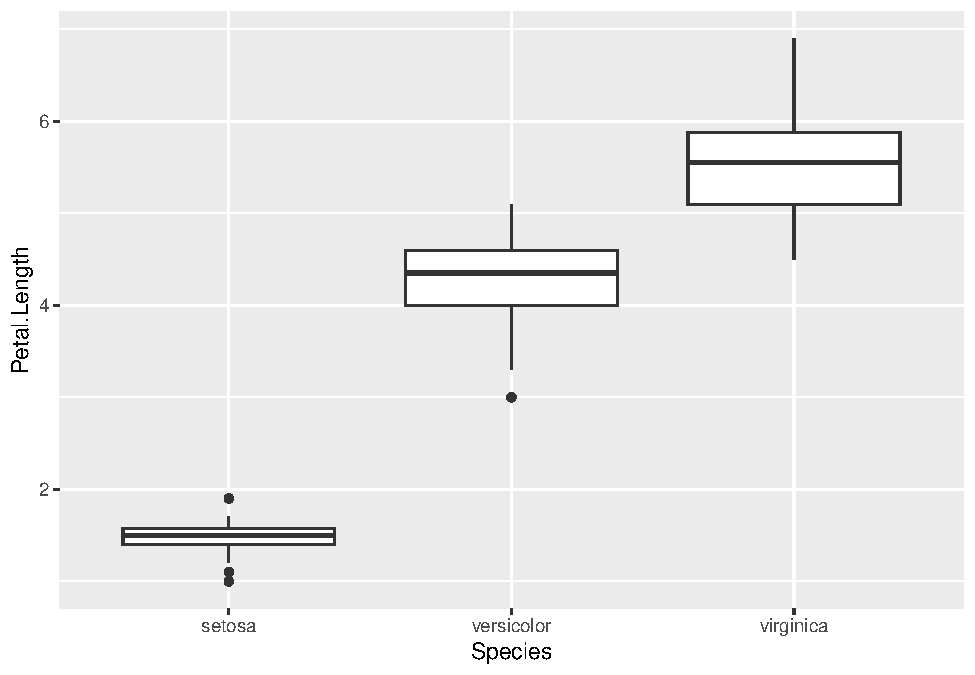
\includegraphics{Untitled_files/figure-latex/unnamed-chunk-19-1.pdf}

\begin{Shaded}
\begin{Highlighting}[]
\DocumentationTok{\#\# scartter plot}
\NormalTok{homerange }\OtherTok{\textless{}{-}} \FunctionTok{read\_csv}\NormalTok{(}\StringTok{"/Users/zhuoyawang/desktop/github/BIS15W2024\_zywang/lab10/data/Tamburelloetal\_HomeRangeDatabase.csv"}\NormalTok{)}
\end{Highlighting}
\end{Shaded}

\begin{verbatim}
## Rows: 569 Columns: 24
## -- Column specification --------------------------------------------------------
## Delimiter: ","
## chr (16): taxon, common.name, class, order, family, genus, species, primarym...
## dbl  (8): mean.mass.g, log10.mass, mean.hra.m2, log10.hra, dimension, preyma...
## 
## i Use `spec()` to retrieve the full column specification for this data.
## i Specify the column types or set `show_col_types = FALSE` to quiet this message.
\end{verbatim}

\begin{Shaded}
\begin{Highlighting}[]
\FunctionTok{ggplot}\NormalTok{(}\AttributeTok{data=}\NormalTok{homerange, }\CommentTok{\#specify the data}
       \AttributeTok{mapping=}\FunctionTok{aes}\NormalTok{(}\AttributeTok{x=}\NormalTok{log10.mass, }\AttributeTok{y=}\NormalTok{log10.hra))}\SpecialCharTok{+} \CommentTok{\#map the aesthetics}
  \FunctionTok{geom\_point}\NormalTok{(}\AttributeTok{na.rm =}\NormalTok{ T)}\SpecialCharTok{+} \CommentTok{\#add the plot type}
  \FunctionTok{geom\_smooth}\NormalTok{(}\AttributeTok{method=}\NormalTok{lm, }\AttributeTok{se=}\NormalTok{T) }\CommentTok{\#add a regression line}
\end{Highlighting}
\end{Shaded}

\begin{verbatim}
## `geom_smooth()` using formula = 'y ~ x'
\end{verbatim}

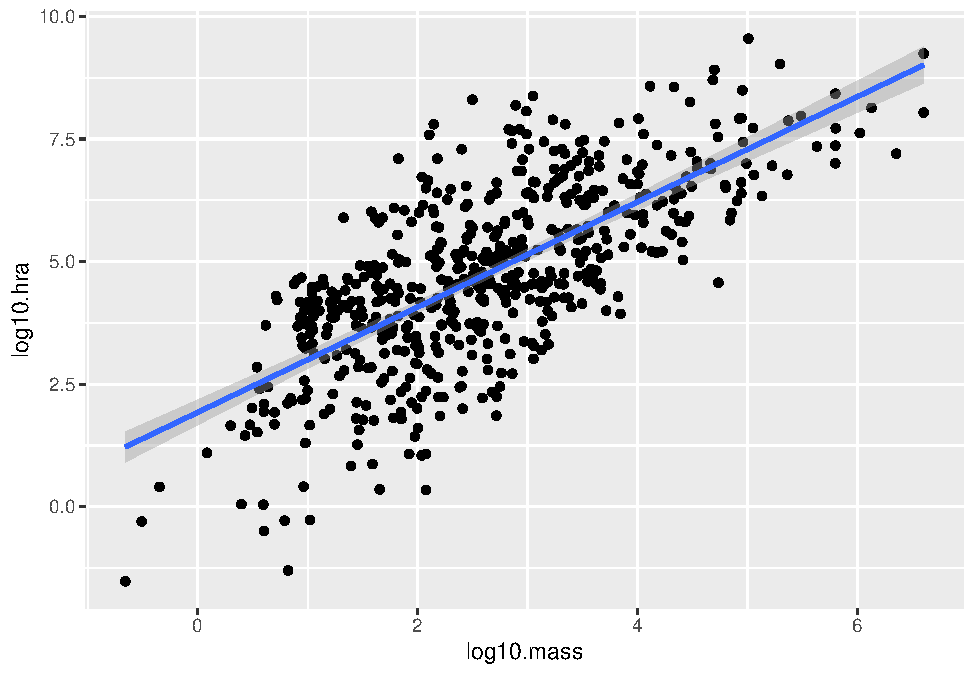
\includegraphics{Untitled_files/figure-latex/unnamed-chunk-19-2.pdf}

\begin{Shaded}
\begin{Highlighting}[]
\CommentTok{\# method=lm, se=F, na.rm=F}
\end{Highlighting}
\end{Shaded}

\hypertarget{bar-plot}{%
\subsubsection{bar plot}\label{bar-plot}}

\begin{Shaded}
\begin{Highlighting}[]
\NormalTok{homerange }\SpecialCharTok{\%\textgreater{}\%} 
  \FunctionTok{ggplot}\NormalTok{(}\FunctionTok{aes}\NormalTok{(}\AttributeTok{x=}\NormalTok{trophic.guild)) }\SpecialCharTok{+} 
  \FunctionTok{geom\_bar}\NormalTok{() }\CommentTok{\#good for counts}
\end{Highlighting}
\end{Shaded}

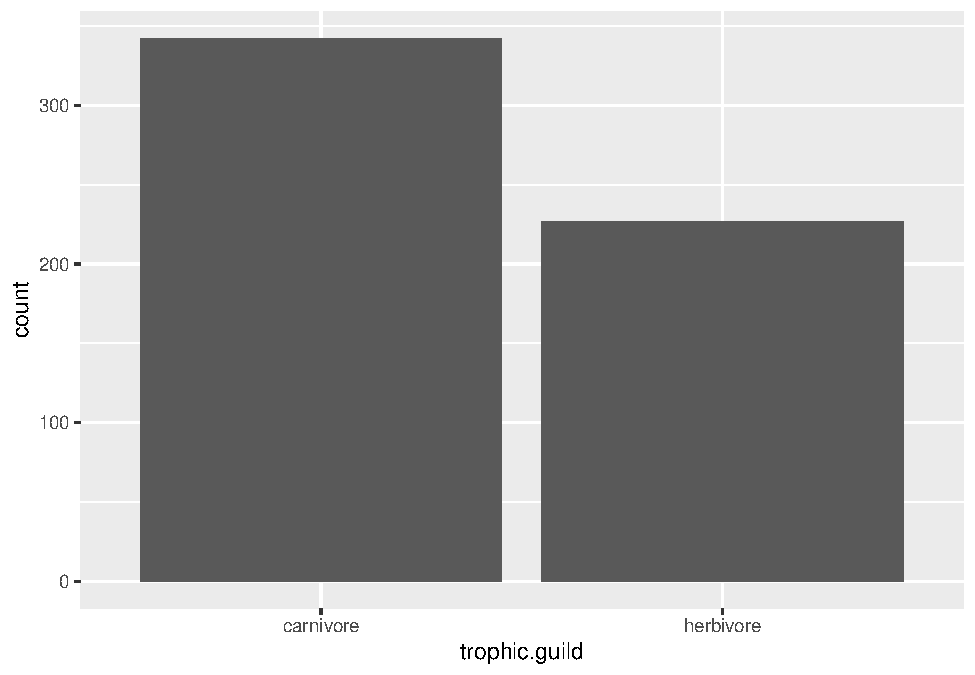
\includegraphics{Untitled_files/figure-latex/unnamed-chunk-20-1.pdf}

\begin{Shaded}
\begin{Highlighting}[]
\NormalTok{homerange }\SpecialCharTok{\%\textgreater{}\%} 
  \FunctionTok{filter}\NormalTok{(family}\SpecialCharTok{==}\StringTok{"salmonidae"}\NormalTok{) }\SpecialCharTok{\%\textgreater{}\%}
  \FunctionTok{select}\NormalTok{(common.name, log10.mass) }\SpecialCharTok{\%\textgreater{}\%} 
  \FunctionTok{ggplot}\NormalTok{(}\FunctionTok{aes}\NormalTok{(}\AttributeTok{x=}\NormalTok{common.name, }\AttributeTok{y=}\NormalTok{log10.mass))}\SpecialCharTok{+} \CommentTok{\#notice the switch in x and y}
  \FunctionTok{geom\_col}\NormalTok{()}\CommentTok{\#+ \# allow to specify the x and y axis}
\end{Highlighting}
\end{Shaded}

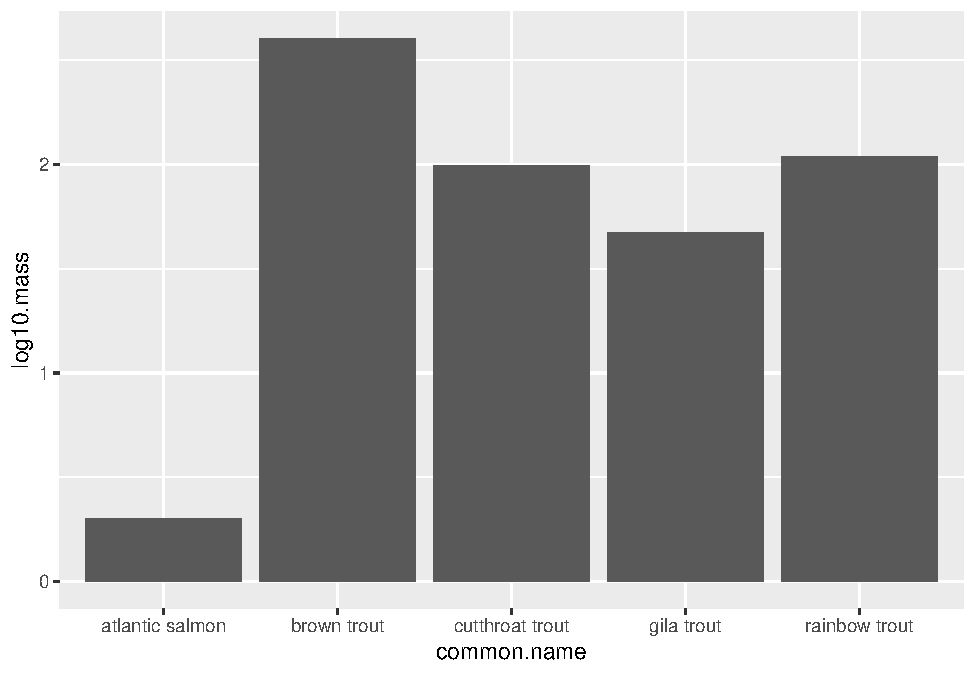
\includegraphics{Untitled_files/figure-latex/unnamed-chunk-21-1.pdf}

\begin{Shaded}
\begin{Highlighting}[]
  \CommentTok{\#coord\_flip() \# change coordination}
\end{Highlighting}
\end{Shaded}

\hypertarget{geom_bar-with-statidentity-statidentity-allows-us-to-map-a-variable-to-the-y-axis-so-that-we-arent-restricted-to-counts.}{%
\subsection{geom\_bar() with stat=``identity'' stat=``identity'' allows
us to map a variable to the y-axis so that we aren't restricted to
counts.}\label{geom_bar-with-statidentity-statidentity-allows-us-to-map-a-variable-to-the-y-axis-so-that-we-arent-restricted-to-counts.}}

\begin{Shaded}
\begin{Highlighting}[]
\NormalTok{homerange }\SpecialCharTok{\%\textgreater{}\%} 
  \FunctionTok{filter}\NormalTok{(family}\SpecialCharTok{==}\StringTok{"salmonidae"}\NormalTok{) }\SpecialCharTok{\%\textgreater{}\%} 
  \FunctionTok{ggplot}\NormalTok{(}\FunctionTok{aes}\NormalTok{(}\AttributeTok{x=}\NormalTok{common.name))}\SpecialCharTok{+}
  \FunctionTok{geom\_bar}\NormalTok{()}
\end{Highlighting}
\end{Shaded}

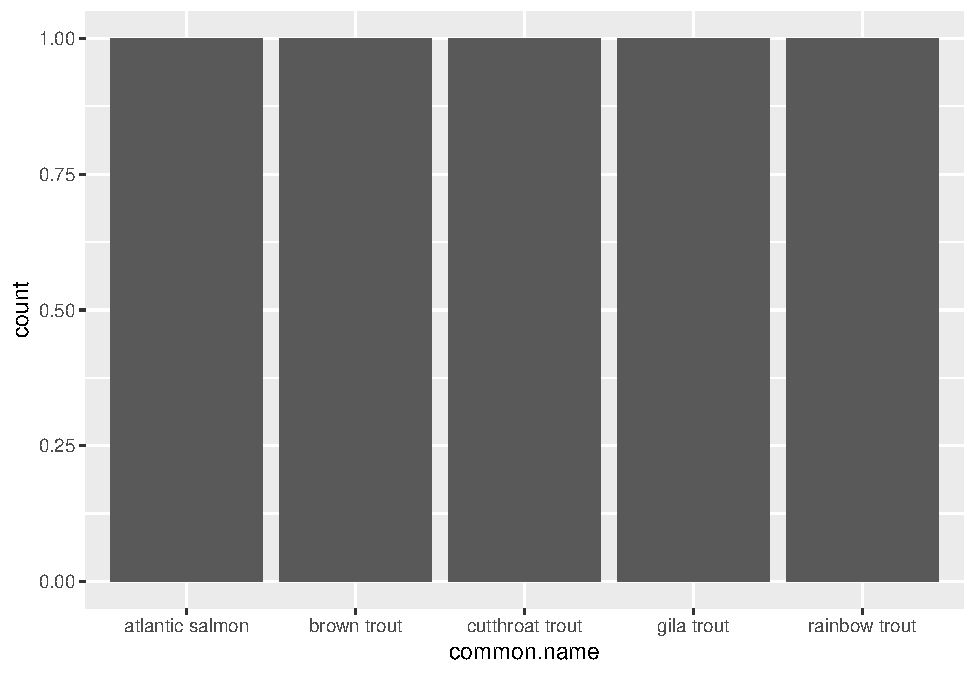
\includegraphics{Untitled_files/figure-latex/unnamed-chunk-22-1.pdf}

\begin{Shaded}
\begin{Highlighting}[]
\NormalTok{homerange }\SpecialCharTok{\%\textgreater{}\%} 
  \FunctionTok{filter}\NormalTok{(family}\SpecialCharTok{==}\StringTok{"salmonidae"}\NormalTok{) }\SpecialCharTok{\%\textgreater{}\%} 
  \FunctionTok{ggplot}\NormalTok{(}\FunctionTok{aes}\NormalTok{(}\AttributeTok{x=}\NormalTok{common.name, }\AttributeTok{y=}\NormalTok{log10.mass))}\SpecialCharTok{+} 
  \FunctionTok{geom\_bar}\NormalTok{(}\AttributeTok{stat=}\StringTok{"identity"}\NormalTok{) }\CommentTok{\# allows to counting y grouped by common name}
\end{Highlighting}
\end{Shaded}

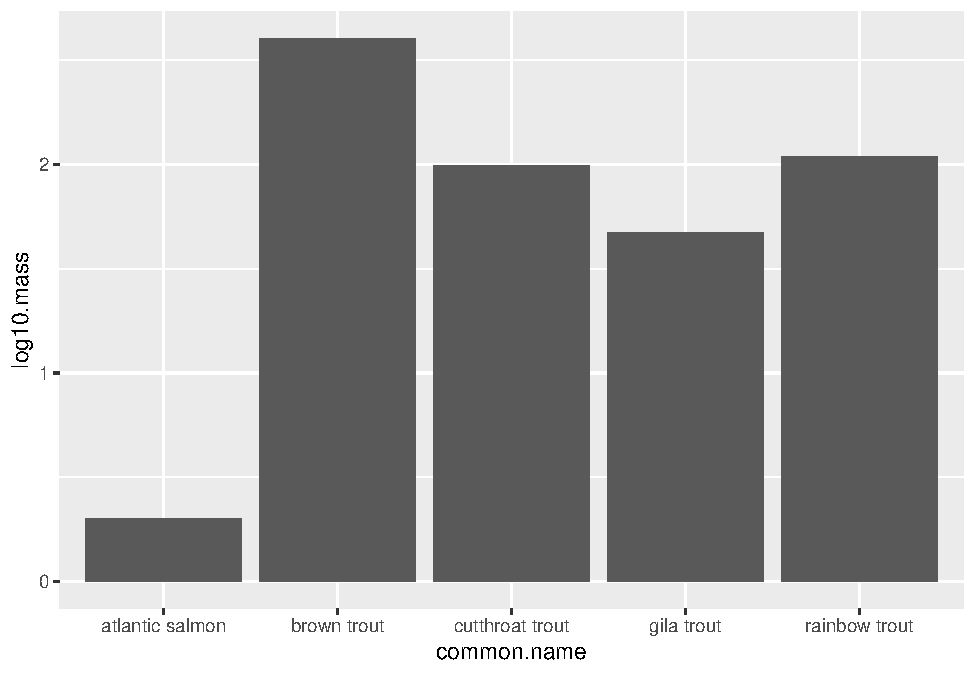
\includegraphics{Untitled_files/figure-latex/unnamed-chunk-23-1.pdf}

\begin{Shaded}
\begin{Highlighting}[]
\FunctionTok{library}\NormalTok{(palmerpenguins)}
\NormalTok{penguins }\SpecialCharTok{\%\textgreater{}\%} 
  \FunctionTok{filter}\NormalTok{(sex }\SpecialCharTok{!=} \StringTok{"NA"}\NormalTok{)}\SpecialCharTok{\%\textgreater{}\%} \CommentTok{\# pull out NAs}
  \FunctionTok{group\_by}\NormalTok{(sex)}\SpecialCharTok{\%\textgreater{}\%}
  \FunctionTok{summarize}\NormalTok{(}\AttributeTok{avg\_bill\_length =} \FunctionTok{mean}\NormalTok{(bill\_length\_mm, }\AttributeTok{na.rm =}\NormalTok{ T))}\SpecialCharTok{\%\textgreater{}\%} 
  \FunctionTok{ggplot}\NormalTok{(}\FunctionTok{aes}\NormalTok{(}\AttributeTok{x=}\NormalTok{sex, }\AttributeTok{y =}\NormalTok{ avg\_bill\_length))}\SpecialCharTok{+}
  \FunctionTok{geom\_col}\NormalTok{()}
\end{Highlighting}
\end{Shaded}

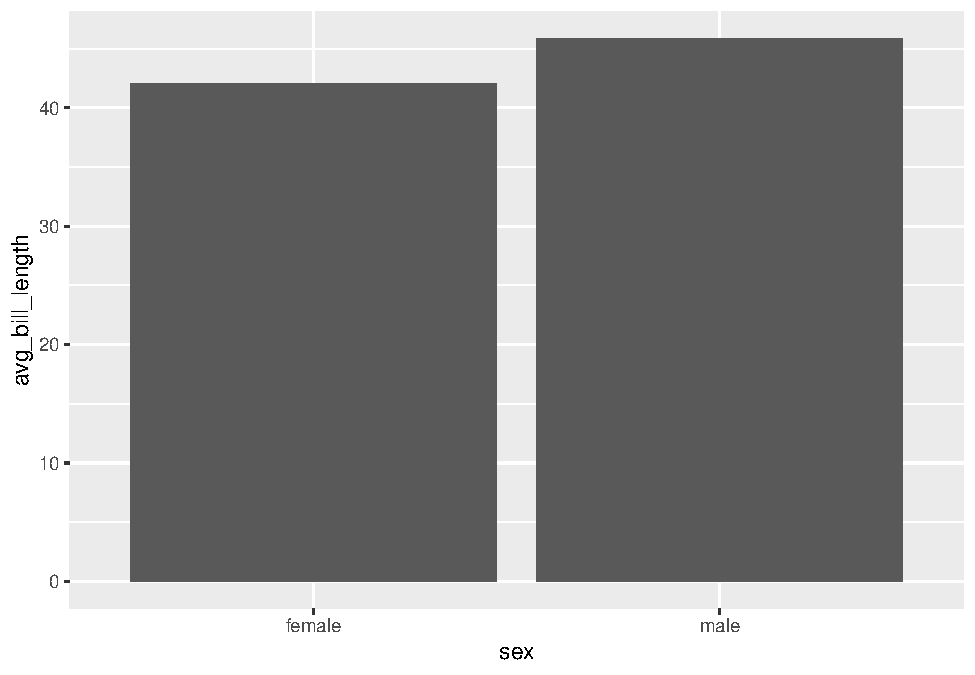
\includegraphics{Untitled_files/figure-latex/unnamed-chunk-24-1.pdf} \#
11.1 Data Visualization: \texttt{ggplot} part 2

\begin{Shaded}
\begin{Highlighting}[]
\FunctionTok{options}\NormalTok{(}\AttributeTok{scipen=}\DecValTok{999}\NormalTok{)}\CommentTok{\#cancels scientific notation for the session}
\FunctionTok{scale\_y\_log10}\NormalTok{() }\CommentTok{\#zoom in plot}
\end{Highlighting}
\end{Shaded}

\begin{verbatim}
## <ScaleContinuousPosition>
##  Range:  
##  Limits:    0 --    1
\end{verbatim}

\begin{Shaded}
\begin{Highlighting}[]
\CommentTok{\#life\_history\%\textgreater{}\%}
\CommentTok{\#  group\_by(order)\%\textgreater{}\%}
\CommentTok{\#  summarize(mean\_mass = mean(mass, na.rm = T))\%\textgreater{}\%}
\CommentTok{\#  ggplot(aes(x = reorder(order, mean\_mass), y = mean\_mass))+ \# allow us to reorder order by mean\_mass}
\CommentTok{\#  geom\_col()+}
\CommentTok{\#  coord\_flip()+}
\CommentTok{\#  scale\_y\_log10()}
\end{Highlighting}
\end{Shaded}

\hypertarget{adjust-position-of-title}{%
\subsubsection{adjust position of
title}\label{adjust-position-of-title}}

\begin{Shaded}
\begin{Highlighting}[]
\CommentTok{\#labs(title="Elephant Age vs. Height", \# add title}
\CommentTok{\#       x="Age(years)", }
\CommentTok{\#       y="Height(cm")+}
\CommentTok{\#  theme(plot.title = element\_text(size = rel(1.5), hjust = 0.5)) \# remove the title to the middle and bigger, hjust is horizontal adjust}
\end{Highlighting}
\end{Shaded}

\hypertarget{filla-common-grouping-option-show-color-based-on-different-group-in-sex}{%
\subsubsection{fill:a common grouping option; show color based on
different group in
sex}\label{filla-common-grouping-option-show-color-based-on-different-group-in-sex}}

\begin{Shaded}
\begin{Highlighting}[]
\CommentTok{\#elephants \%\textgreater{}\% }
\CommentTok{\#  ggplot(aes(x=sex, fill=sex))+}
\CommentTok{\#  geom\_bar()}
\end{Highlighting}
\end{Shaded}

\hypertarget{size-adjusts-the-size-of-points-relative-to-a-continuous-variable.}{%
\subsubsection{size: adjusts the size of points relative to a continuous
variable.}\label{size-adjusts-the-size-of-points-relative-to-a-continuous-variable.}}

\begin{Shaded}
\begin{Highlighting}[]
\NormalTok{life\_history }\SpecialCharTok{\%\textgreater{}\%} 
  \FunctionTok{ggplot}\NormalTok{(}\FunctionTok{aes}\NormalTok{(}\AttributeTok{x=}\NormalTok{gestation, }\AttributeTok{y=}\FunctionTok{log10}\NormalTok{(mass), }\AttributeTok{size=}\NormalTok{mass))}\SpecialCharTok{+}
  \FunctionTok{geom\_point}\NormalTok{(}\AttributeTok{na.rm=}\NormalTok{T)}
\end{Highlighting}
\end{Shaded}

\begin{verbatim}
## Warning in FUN(X[[i]], ...): NaNs produced

## Warning in FUN(X[[i]], ...): NaNs produced
\end{verbatim}

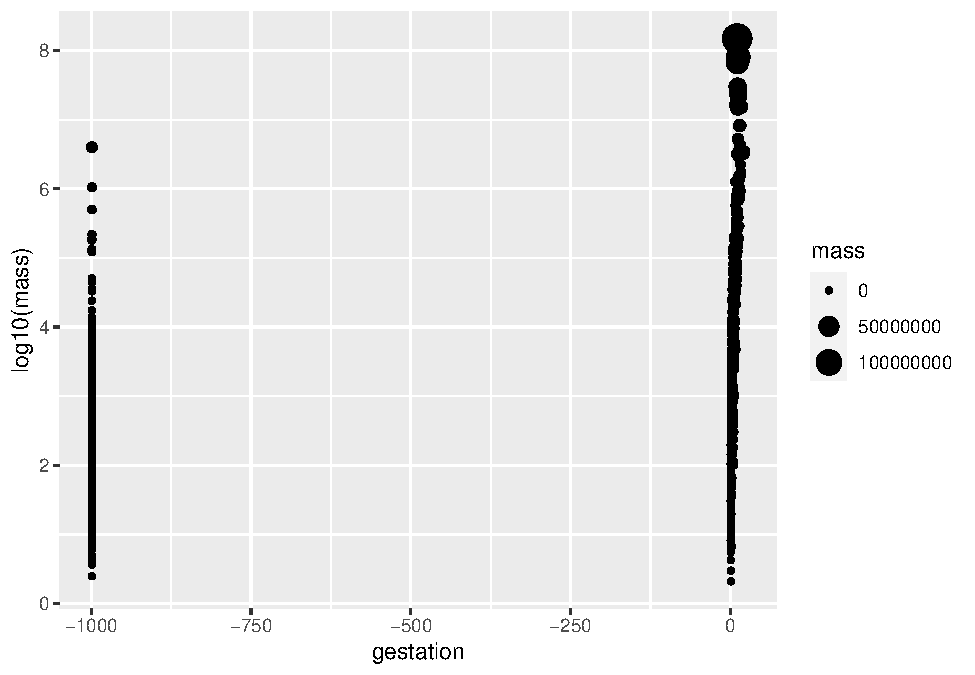
\includegraphics{Untitled_files/figure-latex/unnamed-chunk-28-1.pdf}

\begin{Shaded}
\begin{Highlighting}[]
\CommentTok{\# geom\_point(size=1.25)}
\DocumentationTok{\#\#\#\# adjust point size}


\CommentTok{\# geom\_point(aes(color=thermoregulation), size=1.5) }
\DocumentationTok{\#\#\#\# color the points by a categorical variable.}


\CommentTok{\# geom\_point(aes(shape=thermoregulation, color=thermoregulation), size=1.5) \#\#\#\#\# change shape\& we use color here and not fill because we are not filling a shape}
\end{Highlighting}
\end{Shaded}

\hypertarget{counts-option2-also-a-stacked-bar-plot-that-shows-the-proportion}{%
\subsubsection{counts \& option2 also a stacked bar plot that shows the
proportion}\label{counts-option2-also-a-stacked-bar-plot-that-shows-the-proportion}}

\begin{Shaded}
\begin{Highlighting}[]
\CommentTok{\#option 1}
\NormalTok{homerange }\SpecialCharTok{\%\textgreater{}\%} \FunctionTok{count}\NormalTok{(taxon, }\AttributeTok{sort=}\NormalTok{T)}
\end{Highlighting}
\end{Shaded}

\begin{verbatim}
## # A tibble: 9 x 2
##   taxon             n
##   <chr>         <int>
## 1 mammals         238
## 2 birds           140
## 3 marine fishes    90
## 4 snakes           41
## 5 river fishes     14
## 6 turtles          14
## 7 tortoises        12
## 8 lizards          11
## 9 lake fishes       9
\end{verbatim}

\begin{Shaded}
\begin{Highlighting}[]
\CommentTok{\# option 2}
\NormalTok{homerange }\SpecialCharTok{\%\textgreater{}\%} 
  \FunctionTok{ggplot}\NormalTok{(}\FunctionTok{aes}\NormalTok{(}\AttributeTok{x =}\NormalTok{ taxon, }\AttributeTok{fill =}\NormalTok{ trophic.guild)) }\SpecialCharTok{+} 
  \FunctionTok{geom\_bar}\NormalTok{() }\SpecialCharTok{+}
  \FunctionTok{coord\_flip}\NormalTok{() }\SpecialCharTok{+}
  \FunctionTok{labs}\NormalTok{(}\AttributeTok{title =} \StringTok{"Observations by Taxon in Homerange Data"}\NormalTok{,}
       \AttributeTok{x =} \StringTok{"Taxonomic Group"}\NormalTok{,}
       \AttributeTok{fill =} \StringTok{"Trophic Guild"}\NormalTok{) }\CommentTok{\# legend tittle }
\end{Highlighting}
\end{Shaded}

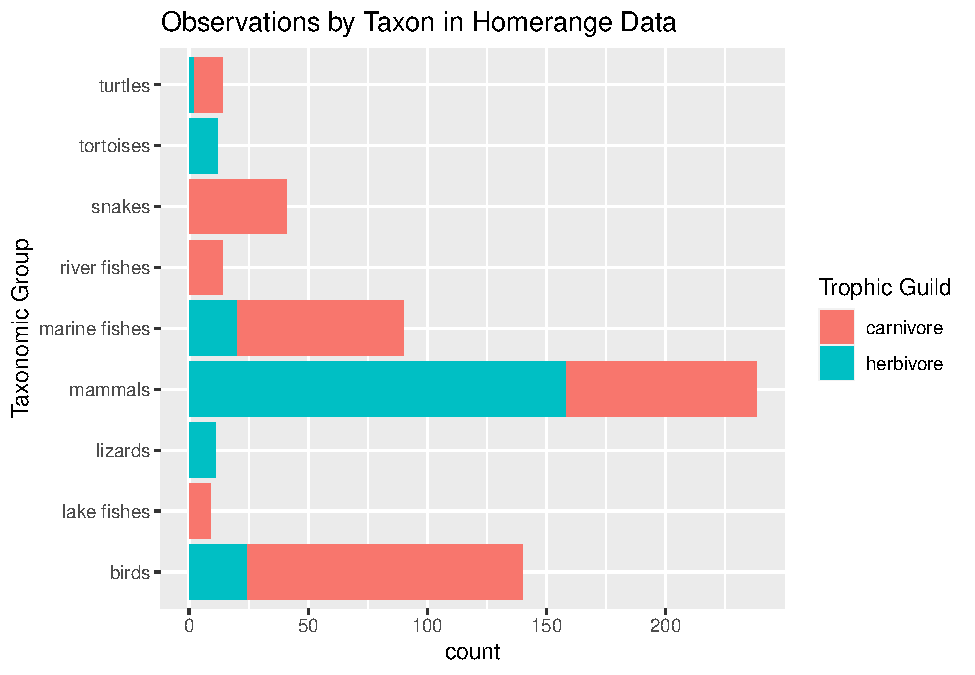
\includegraphics{Untitled_files/figure-latex/unnamed-chunk-30-1.pdf}

\hypertarget{geom_barposition-dodge-side-by-side-bar-plot-for-each-taxon-by-specifying-positiondodge}{%
\subsubsection{geom\_bar(position = ``dodge'')
--\textgreater side-by-side bar plot for each taxon by specifying
position=``dodge''}\label{geom_barposition-dodge-side-by-side-bar-plot-for-each-taxon-by-specifying-positiondodge}}

\begin{Shaded}
\begin{Highlighting}[]
\NormalTok{homerange }\SpecialCharTok{\%\textgreater{}\%} 
  \FunctionTok{ggplot}\NormalTok{(}\FunctionTok{aes}\NormalTok{(}\AttributeTok{x =}\NormalTok{ taxon, }\AttributeTok{fill =}\NormalTok{ trophic.guild)) }\SpecialCharTok{+} 
  \FunctionTok{geom\_bar}\NormalTok{(}\AttributeTok{position =} \StringTok{"dodge"}\NormalTok{) }\SpecialCharTok{+}
  \FunctionTok{coord\_flip}\NormalTok{() }\SpecialCharTok{+}
  \FunctionTok{labs}\NormalTok{(}\AttributeTok{title =} \StringTok{"Observations by Taxon in Homerange Data"}\NormalTok{,}
       \AttributeTok{x =} \StringTok{"Taxonomic Group"}\NormalTok{,}
       \AttributeTok{fill =} \StringTok{"Trophic Guild"}\NormalTok{) }\CommentTok{\# legend tittle }
\end{Highlighting}
\end{Shaded}

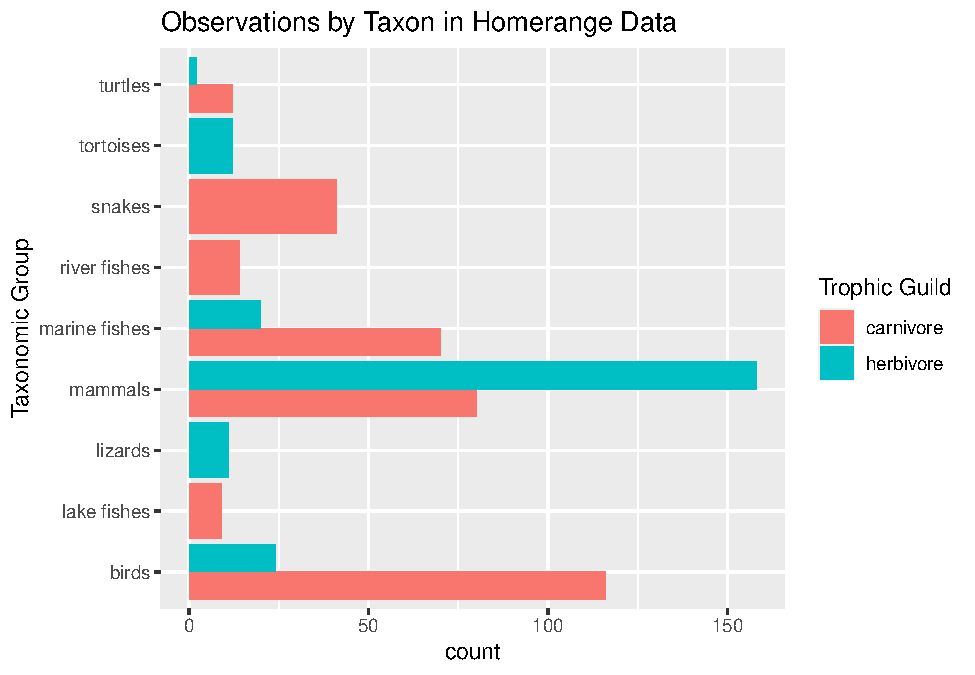
\includegraphics{Untitled_files/figure-latex/unnamed-chunk-31-1.pdf}

\begin{Shaded}
\begin{Highlighting}[]
\CommentTok{\#theme(axis.text.x = element\_text(angle = 60, hjust = 1)) + \#angle is the angle of the text if taxon names are crowded for vertical plot}
\end{Highlighting}
\end{Shaded}

\hypertarget{percentage-bar-plot}{%
\subsubsection{percentage bar plot}\label{percentage-bar-plot}}

\begin{Shaded}
\begin{Highlighting}[]
\NormalTok{homerange }\SpecialCharTok{\%\textgreater{}\%} 
  \FunctionTok{ggplot}\NormalTok{(}\FunctionTok{aes}\NormalTok{(}\AttributeTok{x =}\NormalTok{ taxon, }\AttributeTok{fill =}\NormalTok{ trophic.guild))}\SpecialCharTok{+}
  \FunctionTok{geom\_bar}\NormalTok{(}\AttributeTok{position =} \FunctionTok{position\_fill}\NormalTok{())}\SpecialCharTok{+} 
  \FunctionTok{scale\_y\_continuous}\NormalTok{(}\AttributeTok{labels =}\NormalTok{ scales}\SpecialCharTok{::}\NormalTok{percent)}\SpecialCharTok{+}
  \FunctionTok{coord\_flip}\NormalTok{()}
\end{Highlighting}
\end{Shaded}

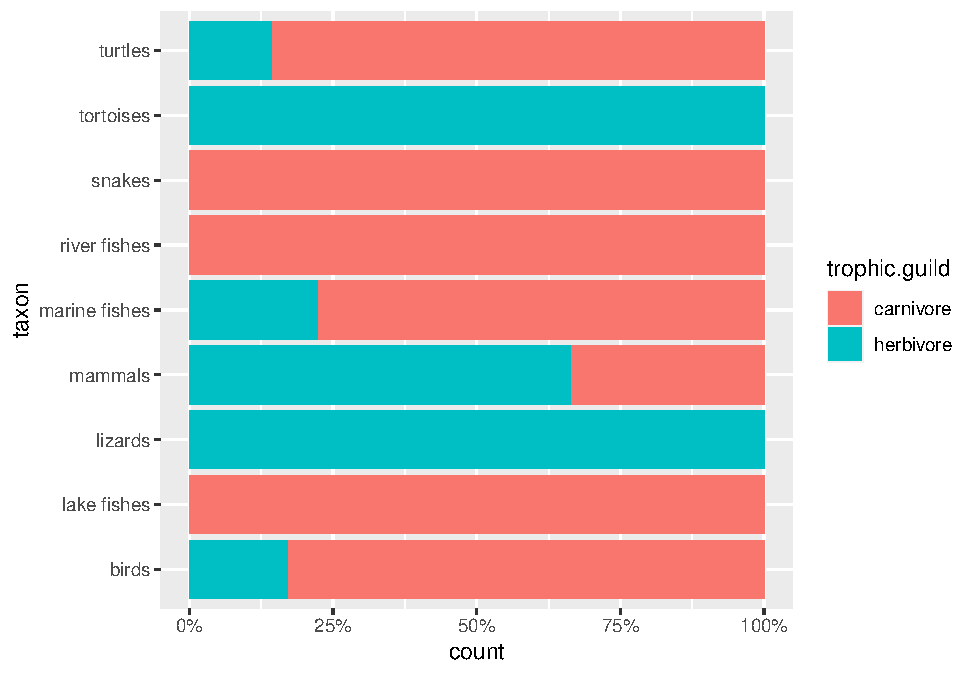
\includegraphics{Untitled_files/figure-latex/unnamed-chunk-32-1.pdf}

\hypertarget{data-visualization-ggplot-part-3}{%
\section{\texorpdfstring{12.1 Data Visualization: \texttt{ggplot} part
3}{12.1 Data Visualization: ggplot part 3}}\label{data-visualization-ggplot-part-3}}

\begin{Shaded}
\begin{Highlighting}[]
\CommentTok{\#library(tidyverse)}
\CommentTok{\#library(RColorBrewer)}
\CommentTok{\#library(paletteer)}
\CommentTok{\#library(janitor)}
\CommentTok{\#deserts \textless{}{-} read\_csv("/Users/zhuoyawang/desktop/github/BIS15W2024\_zywang/lab10/data/surveys\_complete.csv")}
\end{Highlighting}
\end{Shaded}

\hypertarget{line-plot-it-is-need-to-make-year-as.factoryear}{%
\subsection{line plot: it is need to make year
as.factor(year)}\label{line-plot-it-is-need-to-make-year-as.factoryear}}

\begin{Shaded}
\begin{Highlighting}[]
\CommentTok{\#deserts\%\textgreater{}\%}
\CommentTok{\#  filter(species\_id == "DM" | species\_id == "DS")\%\textgreater{}\%}
\CommentTok{\#  mutate(year = as.factor(year))\%\textgreater{}\%}
\CommentTok{\#  group\_by(year, species\_id)\%\textgreater{}\%}
\CommentTok{\#  summarize(n = n(), .groups= "keep")\%\textgreater{}\% \# make it more clean}
\CommentTok{\#  pivot\_wider(names\_from = species\_id, values\_from = n)}
\end{Highlighting}
\end{Shaded}

\begin{Shaded}
\begin{Highlighting}[]
\CommentTok{\#gapminder\%\textgreater{}\%}
\CommentTok{\#  group\_by(year, continent)\%\textgreater{}\%}
\CommentTok{\#  summarize(lc = mean(lifeExp, na.rm = T),.groups= "keep")\%\textgreater{}\%}
\CommentTok{\#  ggplot(aes(x = year, y = lc, color = continent))+}
\CommentTok{\#  geom\_line()+}
\CommentTok{\#  labs(title = "Life Expectancy by Continent",}
\CommentTok{\#       x = "Year",}
\CommentTok{\#       y = "Average Life Expectancy")}
\end{Highlighting}
\end{Shaded}

\hypertarget{histogram-color--boxline-fill--inside-box-bins--box-size}{%
\subsubsection{histogram; color -\textgreater boxline, fill
-\textgreater inside box, bins-\textgreater{} box
size}\label{histogram-color--boxline-fill--inside-box-bins--box-size}}

\begin{Shaded}
\begin{Highlighting}[]
\NormalTok{homerange }\SpecialCharTok{\%\textgreater{}\%} 
  \FunctionTok{ggplot}\NormalTok{(}\FunctionTok{aes}\NormalTok{(}\AttributeTok{x =}\NormalTok{ log10.mass)) }\SpecialCharTok{+}
  \FunctionTok{geom\_histogram}\NormalTok{(}\AttributeTok{color =} \StringTok{"black"}\NormalTok{, }\AttributeTok{fill =} \StringTok{"turquoise4"}\NormalTok{, }\AttributeTok{bins=}\DecValTok{10}\NormalTok{)}\SpecialCharTok{+}
  \FunctionTok{labs}\NormalTok{(}\AttributeTok{title =} \StringTok{"Distribution of Body Mass"}\NormalTok{)}
\end{Highlighting}
\end{Shaded}

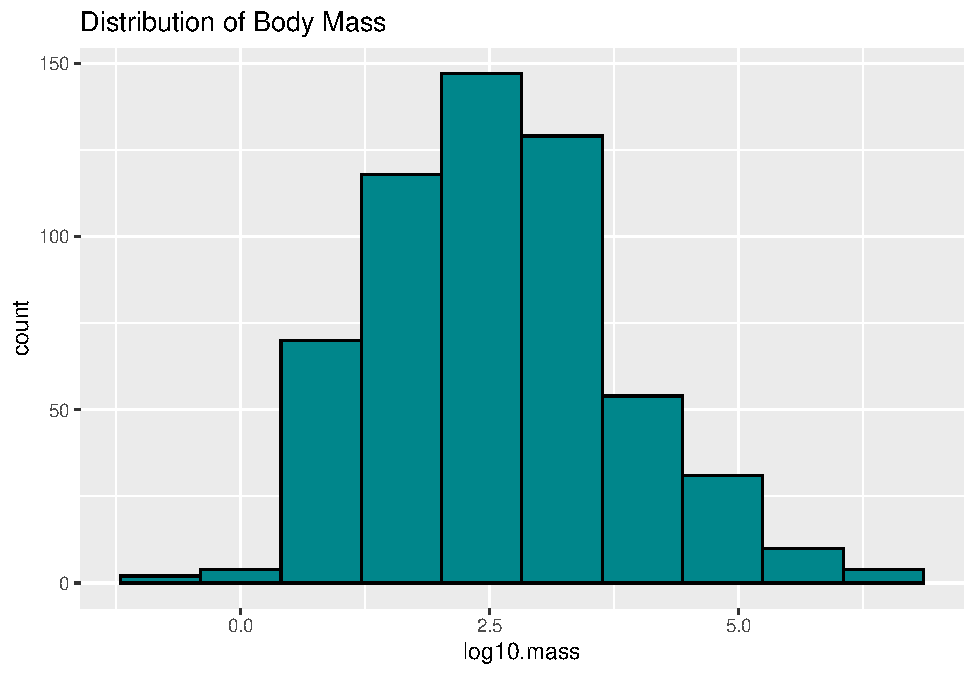
\includegraphics{Untitled_files/figure-latex/unnamed-chunk-36-1.pdf}
\#\#\# Density plot: geom\_density; alpha -\textgreater{} transparency
of plot.

\begin{Shaded}
\begin{Highlighting}[]
\NormalTok{homerange }\SpecialCharTok{\%\textgreater{}\%} 
  \FunctionTok{ggplot}\NormalTok{(}\FunctionTok{aes}\NormalTok{(}\AttributeTok{x =}\NormalTok{ log10.mass)) }\SpecialCharTok{+}
  \FunctionTok{geom\_density}\NormalTok{(}\AttributeTok{fill=}\StringTok{"deepskyblue4"}\NormalTok{, }\AttributeTok{alpha  =}\FloatTok{0.4}\NormalTok{, }\AttributeTok{color =} \StringTok{"black"}\NormalTok{)}\SpecialCharTok{+} \CommentTok{\#alpha is the transparency}
  \FunctionTok{labs}\NormalTok{(}\AttributeTok{title =} \StringTok{"Distribution of Body Mass"}\NormalTok{)}
\end{Highlighting}
\end{Shaded}

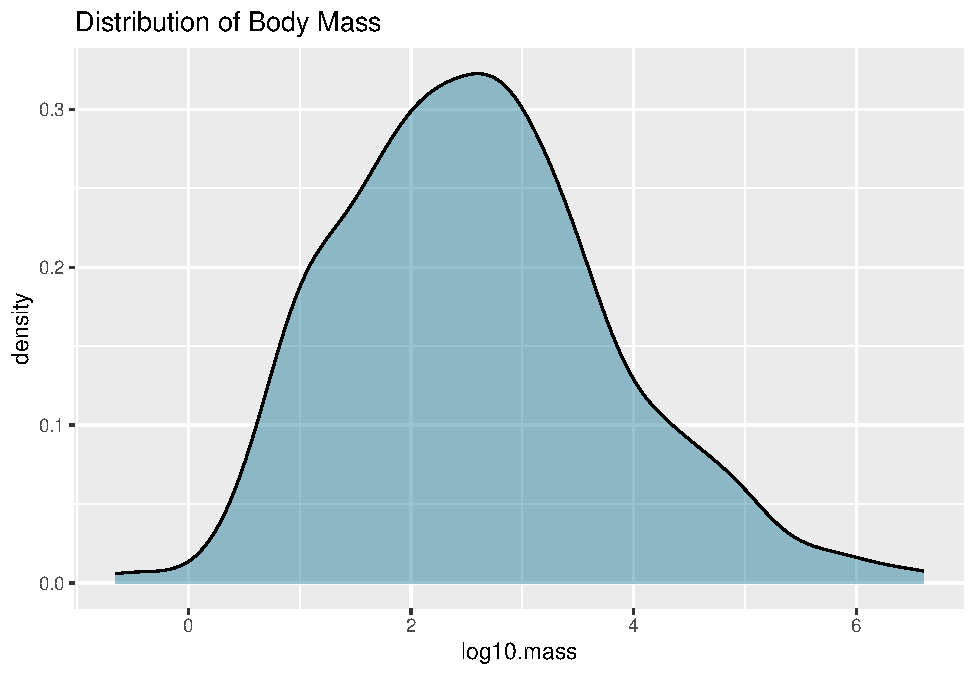
\includegraphics{Untitled_files/figure-latex/unnamed-chunk-37-1.pdf}

\begin{Shaded}
\begin{Highlighting}[]
\NormalTok{homerange }\SpecialCharTok{\%\textgreater{}\%} 
  \FunctionTok{ggplot}\NormalTok{(}\FunctionTok{aes}\NormalTok{(}\AttributeTok{x=}\NormalTok{log10.mass)) }\SpecialCharTok{+}
  \FunctionTok{geom\_histogram}\NormalTok{(}\FunctionTok{aes}\NormalTok{(}\AttributeTok{y =} \FunctionTok{after\_stat}\NormalTok{(density)), }\AttributeTok{fill =} \StringTok{"deepskyblue4"}\NormalTok{, }\AttributeTok{alpha =} \FloatTok{0.4}\NormalTok{, }\AttributeTok{color =} \StringTok{"black"}\NormalTok{)}\SpecialCharTok{+}
  \FunctionTok{geom\_density}\NormalTok{(}\AttributeTok{color =} \StringTok{"red"}\NormalTok{)}\SpecialCharTok{+} \CommentTok{\# density line}
  \FunctionTok{labs}\NormalTok{(}\AttributeTok{title =} \StringTok{"Distribution of Body Mass"}\NormalTok{)}
\end{Highlighting}
\end{Shaded}

\begin{verbatim}
## `stat_bin()` using `bins = 30`. Pick better value with `binwidth`.
\end{verbatim}

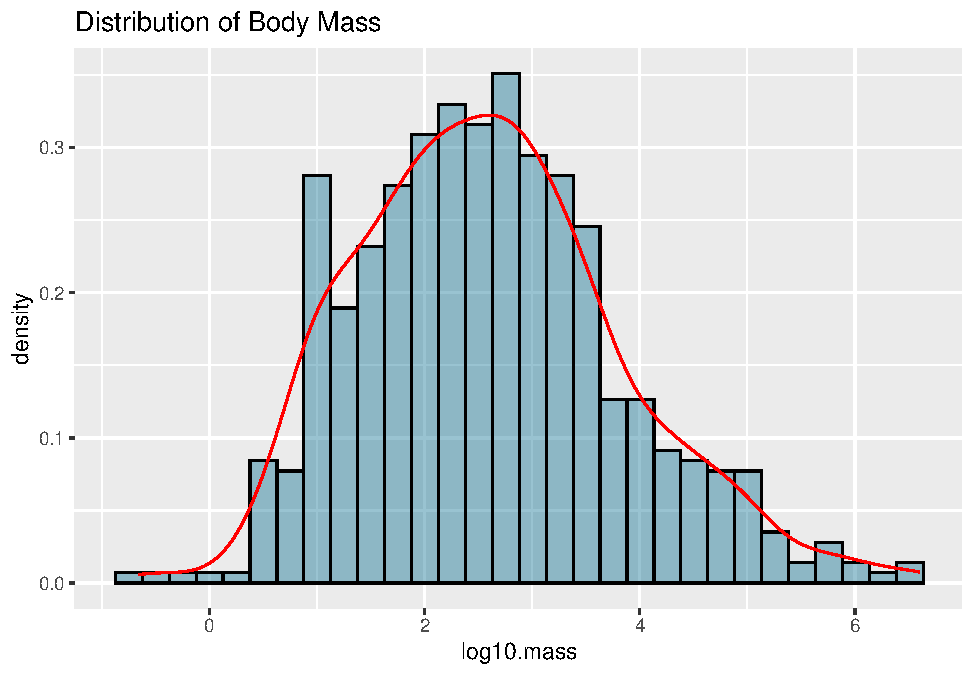
\includegraphics{Untitled_files/figure-latex/unnamed-chunk-38-1.pdf}

\hypertarget{section}{%
\section{12.2}\label{section}}

\begin{Shaded}
\begin{Highlighting}[]
\NormalTok{p }\OtherTok{\textless{}{-}}\NormalTok{ homerange }\SpecialCharTok{\%\textgreater{}\%} 
  \FunctionTok{ggplot}\NormalTok{(}\FunctionTok{aes}\NormalTok{(}\AttributeTok{x=}\NormalTok{taxon, }\AttributeTok{fill=}\NormalTok{trophic.guild))}\SpecialCharTok{+}
  \FunctionTok{geom\_bar}\NormalTok{(}\AttributeTok{na.rm=}\NormalTok{T, }\AttributeTok{position=}\StringTok{"dodge"}\NormalTok{);p}
\end{Highlighting}
\end{Shaded}

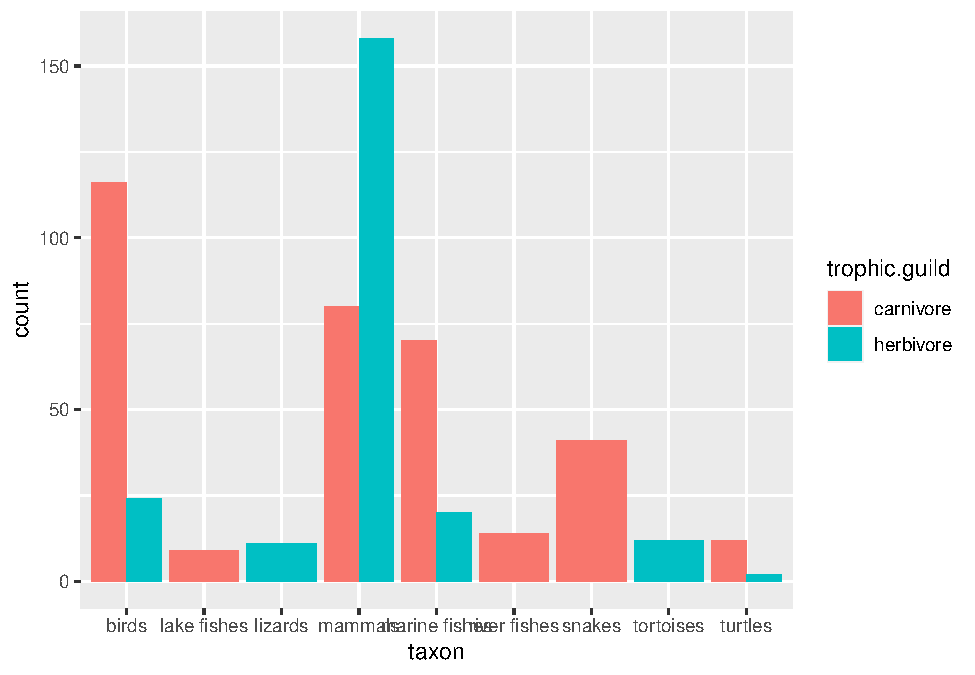
\includegraphics{Untitled_files/figure-latex/unnamed-chunk-39-1.pdf}

\hypertarget{linedraw-adding-another-layer}{%
\subsubsection{linedraw : adding another
layer}\label{linedraw-adding-another-layer}}

\begin{Shaded}
\begin{Highlighting}[]
\NormalTok{p }\SpecialCharTok{+} \FunctionTok{theme\_linedraw}\NormalTok{()}\SpecialCharTok{+}
  \FunctionTok{theme}\NormalTok{(}\AttributeTok{axis.text.x =} \FunctionTok{element\_text}\NormalTok{(}\AttributeTok{angle =} \DecValTok{60}\NormalTok{, }\AttributeTok{hjust=}\DecValTok{1}\NormalTok{))}\SpecialCharTok{+}
  \FunctionTok{labs}\NormalTok{(}\AttributeTok{title =} \StringTok{"Observations by Taxon in Homerange Data"}\NormalTok{,}
       \AttributeTok{x =} \ConstantTok{NULL}\NormalTok{,}
       \AttributeTok{y=} \StringTok{"n"}\NormalTok{,}
       \AttributeTok{fill=} \StringTok{"Trophic Guild"}\NormalTok{)}
\end{Highlighting}
\end{Shaded}

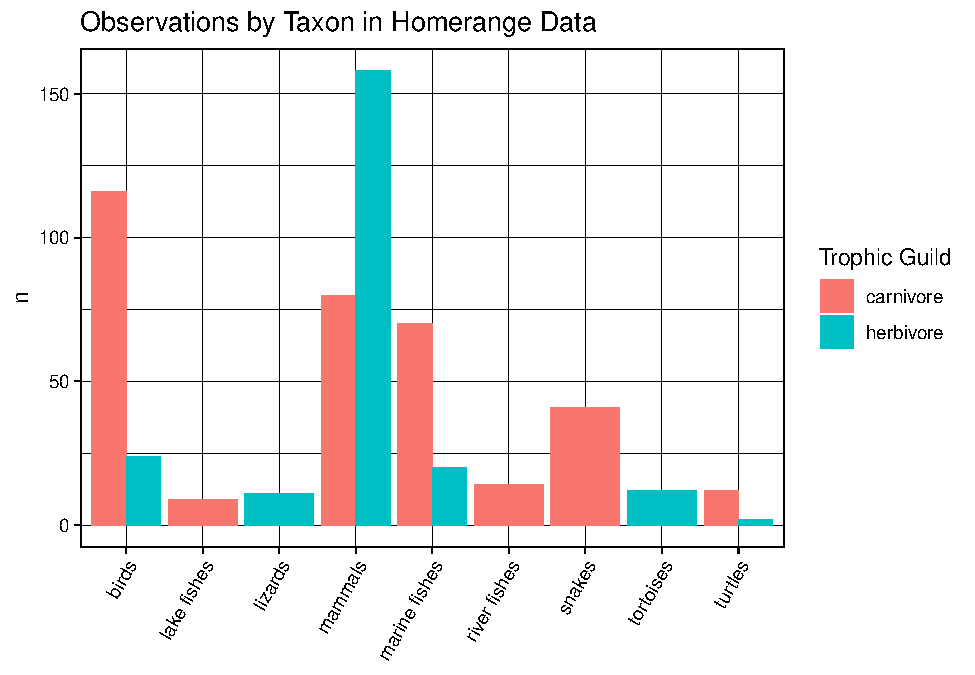
\includegraphics{Untitled_files/figure-latex/unnamed-chunk-40-1.pdf}

\begin{Shaded}
\begin{Highlighting}[]
\NormalTok{q }\OtherTok{\textless{}{-}}\NormalTok{ homerange }\SpecialCharTok{\%\textgreater{}\%} 
  \FunctionTok{ggplot}\NormalTok{(}\FunctionTok{aes}\NormalTok{(}\AttributeTok{x=}\NormalTok{log10.mass, }\AttributeTok{y=}\NormalTok{log10.preymass, }\AttributeTok{color=}\NormalTok{taxon))}\SpecialCharTok{+}
  \FunctionTok{geom\_point}\NormalTok{(}\AttributeTok{na.rm=}\NormalTok{T);q}
\end{Highlighting}
\end{Shaded}

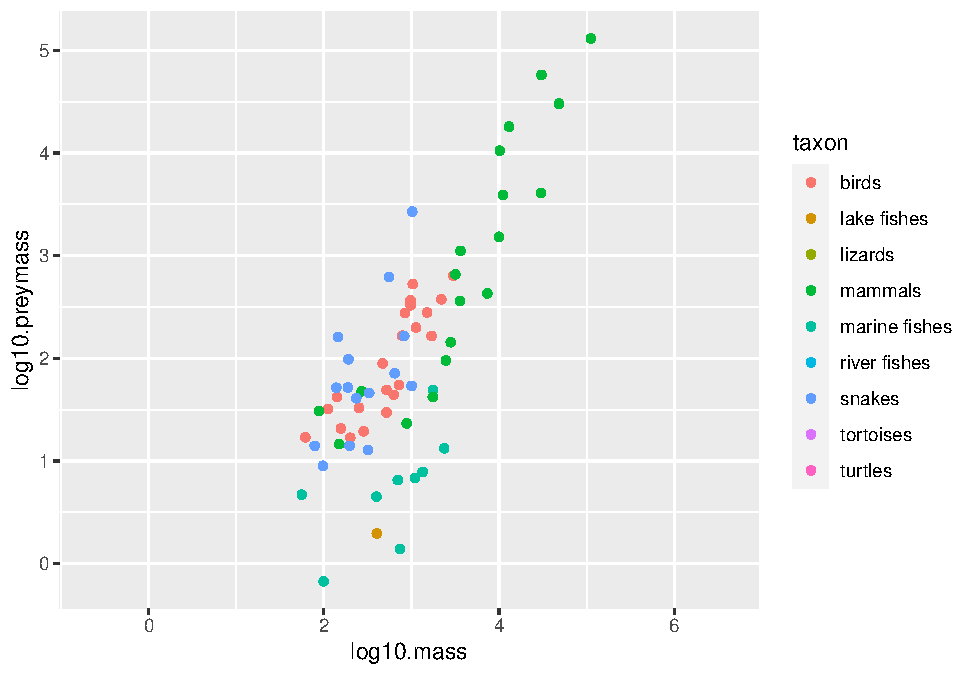
\includegraphics{Untitled_files/figure-latex/unnamed-chunk-41-1.pdf}

\begin{Shaded}
\begin{Highlighting}[]
\NormalTok{q }\SpecialCharTok{+} \FunctionTok{theme\_classic}\NormalTok{()}
\end{Highlighting}
\end{Shaded}

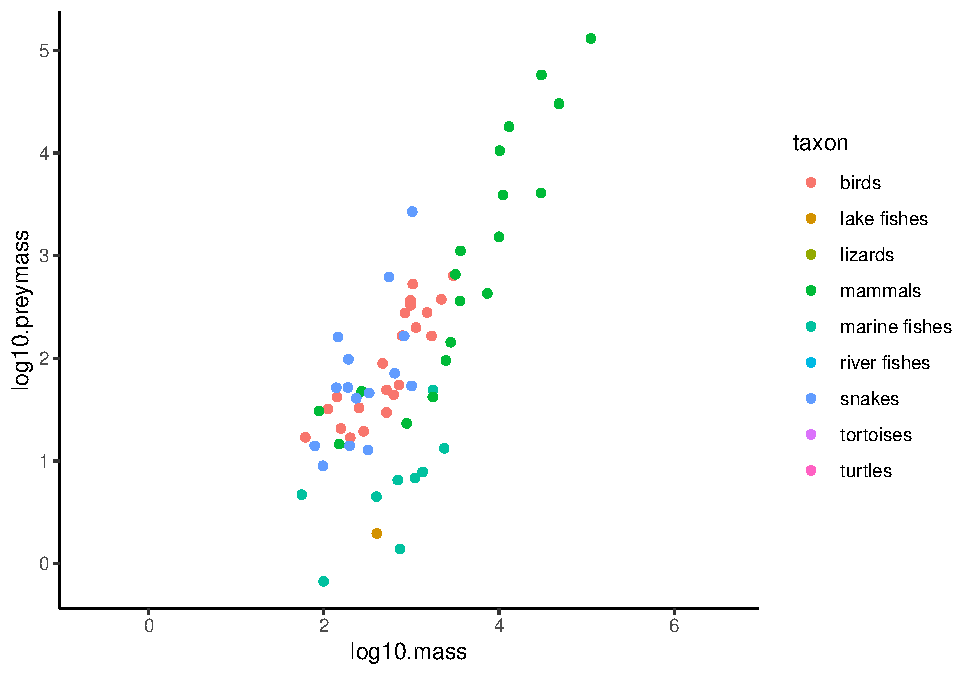
\includegraphics{Untitled_files/figure-latex/unnamed-chunk-42-1.pdf}

\hypertarget{faceting}{%
\subsection{Faceting}\label{faceting}}

\begin{Shaded}
\begin{Highlighting}[]
\NormalTok{homerange }\SpecialCharTok{\%\textgreater{}\%} 
  \FunctionTok{ggplot}\NormalTok{(}\FunctionTok{aes}\NormalTok{(}\AttributeTok{x=}\NormalTok{taxon, }\AttributeTok{y=}\NormalTok{log10.mass))}\SpecialCharTok{+}
  \FunctionTok{geom\_boxplot}\NormalTok{()}\SpecialCharTok{+}
  \FunctionTok{theme}\NormalTok{(}\AttributeTok{axis.text.x =} \FunctionTok{element\_text}\NormalTok{(}\AttributeTok{angle =} \DecValTok{60}\NormalTok{, }\AttributeTok{hjust=}\DecValTok{1}\NormalTok{))}
\end{Highlighting}
\end{Shaded}

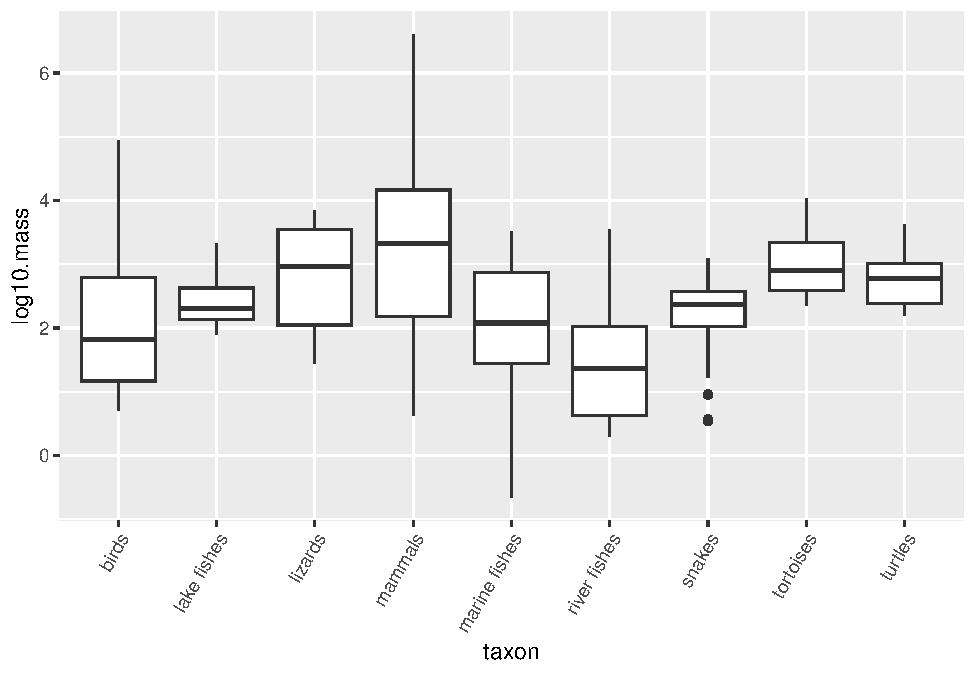
\includegraphics{Untitled_files/figure-latex/unnamed-chunk-43-1.pdf}

\hypertarget{facet_wrap-makes-a-ribbon-of-panels-by-a-specified-categorical-variable}{%
\subsection{facet\_wrap makes a ribbon of panels by a specified
categorical
variable}\label{facet_wrap-makes-a-ribbon-of-panels-by-a-specified-categorical-variable}}

\begin{Shaded}
\begin{Highlighting}[]
\NormalTok{homerange }\SpecialCharTok{\%\textgreater{}\%} 
  \FunctionTok{ggplot}\NormalTok{(}\FunctionTok{aes}\NormalTok{(}\AttributeTok{x=}\NormalTok{taxon, }\AttributeTok{y=}\NormalTok{log10.mass))}\SpecialCharTok{+}
  \FunctionTok{geom\_boxplot}\NormalTok{()}\SpecialCharTok{+}
  \FunctionTok{facet\_wrap}\NormalTok{(}\SpecialCharTok{\textasciitilde{}}\NormalTok{trophic.guild, }\AttributeTok{ncol=}\DecValTok{2}\NormalTok{)}\SpecialCharTok{+}
  \FunctionTok{theme}\NormalTok{(}\AttributeTok{axis.text.x =} \FunctionTok{element\_text}\NormalTok{(}\AttributeTok{angle =} \DecValTok{60}\NormalTok{, }\AttributeTok{hjust=}\DecValTok{1}\NormalTok{))}
\end{Highlighting}
\end{Shaded}

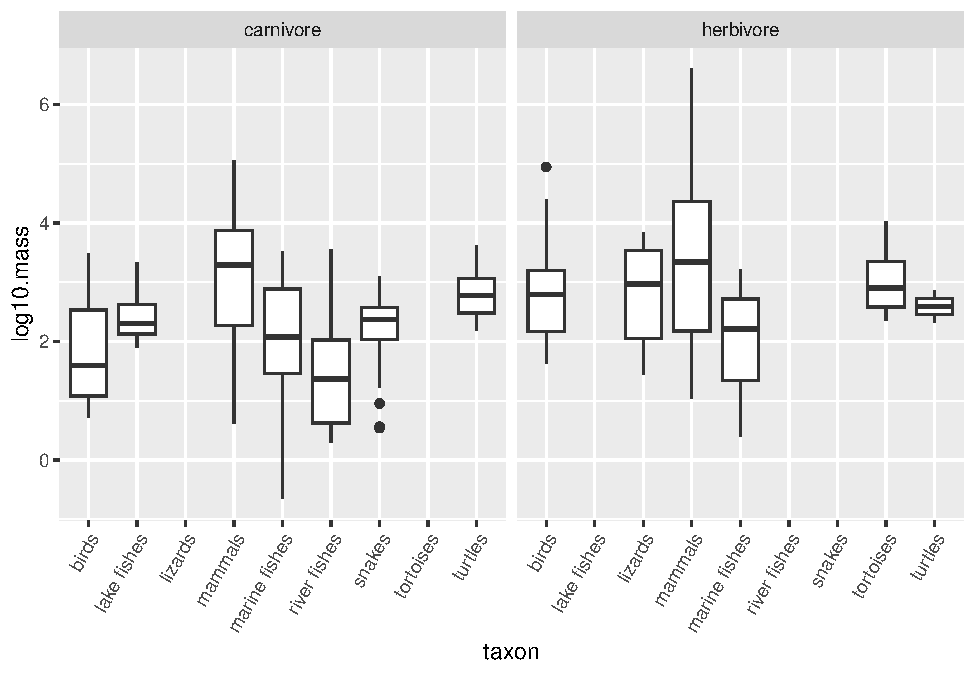
\includegraphics{Untitled_files/figure-latex/unnamed-chunk-44-1.pdf}

\hypertarget{facet_grid-control-over-the-faceted-variable-it-can-be-arranged-in-rows-or-columns.}{%
\subsection{facet\_grid: control over the faceted variable; it can be
arranged in rows or
columns.}\label{facet_grid-control-over-the-faceted-variable-it-can-be-arranged-in-rows-or-columns.}}

\hypertarget{rowscolumns.}{%
\subsection{rows\textasciitilde columns.}\label{rowscolumns.}}

\begin{Shaded}
\begin{Highlighting}[]
\NormalTok{homerange }\SpecialCharTok{\%\textgreater{}\%} 
  \FunctionTok{ggplot}\NormalTok{(}\FunctionTok{aes}\NormalTok{(}\AttributeTok{x=}\NormalTok{taxon, }\AttributeTok{y=}\NormalTok{log10.mass))}\SpecialCharTok{+}
  \FunctionTok{geom\_boxplot}\NormalTok{()}\SpecialCharTok{+}
  \FunctionTok{facet\_grid}\NormalTok{(trophic.guild}\SpecialCharTok{\textasciitilde{}}\NormalTok{.)}\SpecialCharTok{+} \CommentTok{\# in rows}
  \FunctionTok{theme}\NormalTok{(}\AttributeTok{axis.text.x =} \FunctionTok{element\_text}\NormalTok{(}\AttributeTok{angle =} \DecValTok{60}\NormalTok{, }\AttributeTok{hjust=}\DecValTok{1}\NormalTok{))}
\end{Highlighting}
\end{Shaded}

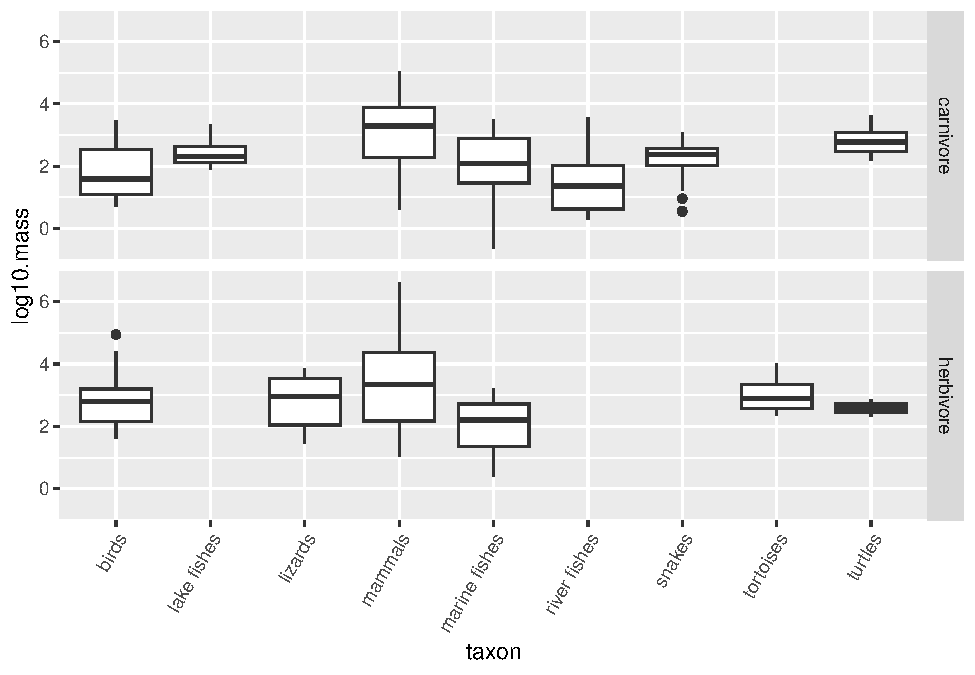
\includegraphics{Untitled_files/figure-latex/unnamed-chunk-45-1.pdf}

\begin{Shaded}
\begin{Highlighting}[]
\NormalTok{homerange }\SpecialCharTok{\%\textgreater{}\%} 
  \FunctionTok{ggplot}\NormalTok{(}\FunctionTok{aes}\NormalTok{(}\AttributeTok{x=}\NormalTok{taxon, }\AttributeTok{y=}\NormalTok{log10.mass))}\SpecialCharTok{+}
  \FunctionTok{geom\_boxplot}\NormalTok{()}\SpecialCharTok{+}
  \FunctionTok{facet\_grid}\NormalTok{(.}\SpecialCharTok{\textasciitilde{}}\NormalTok{trophic.guild)}\SpecialCharTok{+} \CommentTok{\# in col }
  \FunctionTok{theme}\NormalTok{(}\AttributeTok{axis.text.x =} \FunctionTok{element\_text}\NormalTok{(}\AttributeTok{angle =} \DecValTok{60}\NormalTok{, }\AttributeTok{hjust=}\DecValTok{1}\NormalTok{))}
\end{Highlighting}
\end{Shaded}

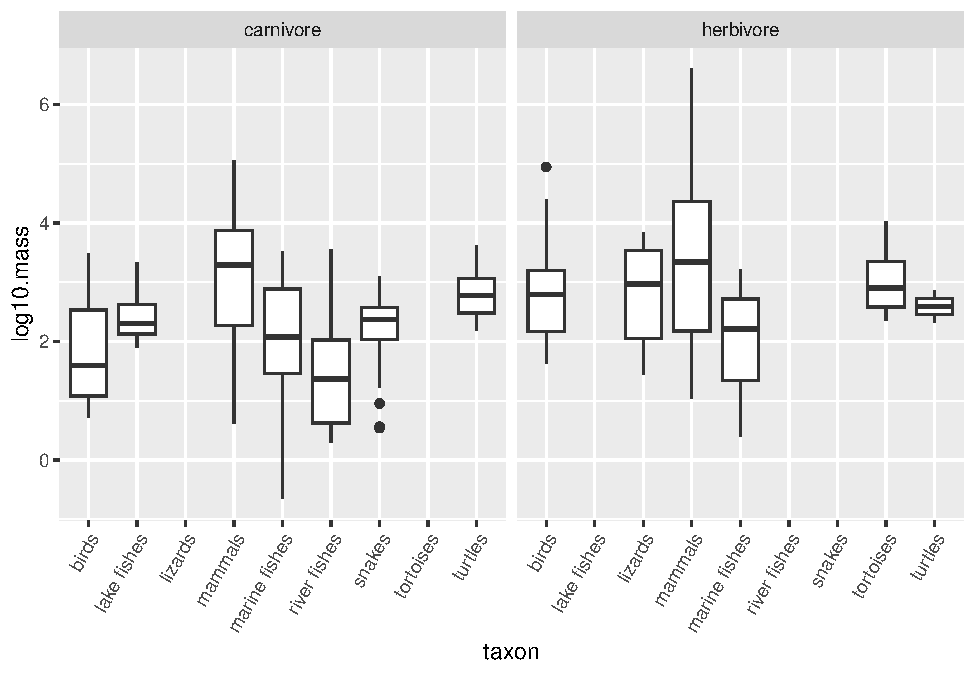
\includegraphics{Untitled_files/figure-latex/unnamed-chunk-46-1.pdf}

\begin{Shaded}
\begin{Highlighting}[]
\NormalTok{homerange }\SpecialCharTok{\%\textgreater{}\%} 
  \FunctionTok{ggplot}\NormalTok{(}\FunctionTok{aes}\NormalTok{(}\AttributeTok{x=}\NormalTok{taxon, }\AttributeTok{y=}\NormalTok{log10.mass))}\SpecialCharTok{+}
  \FunctionTok{geom\_boxplot}\NormalTok{()}\SpecialCharTok{+}
  \FunctionTok{facet\_grid}\NormalTok{(trophic.guild}\SpecialCharTok{\textasciitilde{}}\NormalTok{thermoregulation)}\SpecialCharTok{+}
  \FunctionTok{theme}\NormalTok{(}\AttributeTok{axis.text.x =} \FunctionTok{element\_text}\NormalTok{(}\AttributeTok{angle =} \DecValTok{60}\NormalTok{, }\AttributeTok{hjust=}\DecValTok{1}\NormalTok{))}
\end{Highlighting}
\end{Shaded}

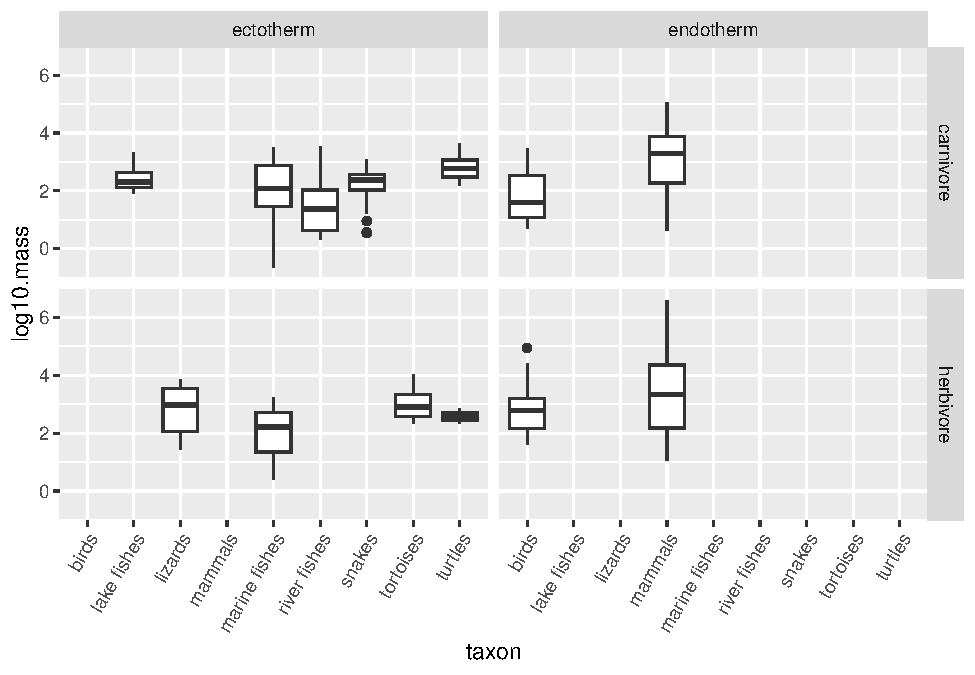
\includegraphics{Untitled_files/figure-latex/unnamed-chunk-47-1.pdf}

\hypertarget{hw11-review}{%
\subsection{HW11 review}\label{hw11-review}}

\begin{Shaded}
\begin{Highlighting}[]
\CommentTok{\#top5 \textless{}{-} gapminder\%\textgreater{}\%}
\CommentTok{\#  filter(year \%in\% c(1952, 2007))\%\textgreater{}\%}
\CommentTok{\#  group\_by(country)\%\textgreater{}\%}
\CommentTok{\#  summarize(start = first(pop),}
\CommentTok{\#            end = last(pop),}
\CommentTok{\#            pop\_growth = (end{-}start))\%\textgreater{}\%}
\CommentTok{\#  arrange(desc(pop\_growth))\%\textgreater{}\%}
\CommentTok{\#  top\_n(5,pop\_growth);top5}
\end{Highlighting}
\end{Shaded}

\begin{Shaded}
\begin{Highlighting}[]
\CommentTok{\#gapminder\%\textgreater{}\%}
\CommentTok{\#  filter(year \%in\%c(1952, 2007) \& country \%in\% top5$country)\%\textgreater{}\%}
\CommentTok{\#  ggplot(aes(x = reorder(country, pop), y = pop, fill = year))+}
\CommentTok{\#  geom\_bar(stat = "identity", position = "dodge")+}
\CommentTok{\#  coord\_flip()+}
\CommentTok{\#  labs(title = "Top 5 Population Growth Countries", x = "population", y = "country")}
\end{Highlighting}
\end{Shaded}


\end{document}
